% !TeX root = RJwrapper.tex
\title{Variety and Mainstays of the R Developer Community}


\author{by Lijin Zhang, Xueyang Li, and Zhiyong Zhang}

\maketitle

\abstract{%
The thriving developer community has a significant impact on the widespread use of R software. To better understand this community, we conducted a study analyzing all R packages available on CRAN. We identified the most popular topics of R packages by text mining the package descriptions. Additionally, using network centrality measures, we discovered the important packages in the package dependency network and influential developers in the global R community. Our analysis showed that among the 20 topics identified in the topic model, \emph{Data Import, Export, and Wrangling}, as well as \emph{Data Visualization, Result Presentation, and Interactive Web Applications}, were particularly popular among influential packages and developers. These findings provide valuable insights into the R community.
}

\section{Introduction}

Initially started as a personal project by Ross Ihaka and Robert Gentleman \citep{ihaka1996r}, R has evolved into one of the most widely used and powerful software packages in the field of data science. It is used across a wide range of academic fields and industries.  For example, \citet{lai2019evaluating} showed that 58\% of the papers from 30 ecology journals in 2017 reported using R for data analysis. Another example is Bioconductor \citep{gentleman2004bioconductor}, a popular R software repository for computational biology and bioinformatics, which has over 2,000 R packages for genetic data analysis. Moreover, \CRANpkg{ggplot2} \citep{wickham2011ggplot2}, a well-known R package for data visualization, has been cited more than 30,000 times. Courses teaching R are also in high demand in data science programs \citep{zhang2021data}. \citet{fox2016r} analyzed the papers published in the Journal of Statistical Software (JSS) between 1996 and 2016, and found that 75\% of the articles were about R, which demonstrated the dominance of R software projects in JSS. 

The R developer community plays an important role in maintaining a healthy ecosystem of R packages and increasing R's popularity (\citealp{RJ-2020-028}; \citealp{tippmann2015programming}). The R ecosystem comprises of the base packages developed by the R Core team and user-contributed packages \citep{german2013evolution}. The Comprehensive R Archive Network (CRAN) is a well-known package repository. \citet{fox2009aspects} suggested that the CRAN package archive is probably the most important driving force for the growing usage of R. The package system provides essential tools for users to develop packages and promotes the sharing of newly-developed methods and ideas throughout the community. \citet{fox2009aspects} found that the growth of CRAN packages from 2000 to 2009 was approximately exponential. Since then, the number of new CRAN packages has slowed down a bit, but has otherwise maintained a steady pace \citep{fox2016r}.  As of 27th November 2022, there are 18898 packages available on CRAN, more than eight times of the number in 2009.


As the number of CRAN packages increases, the flat organization of these packages \citep{fox2016r} makes it difficult for user to identify popular and important packages on CRAN.  \citet{RJ-2018-058} suggested that the huge size of the CRAN package archive has already made it difficult for users to understand the merits of packages and the relationships among packages. Although some resources such as CRAN Task Views \citep{zeileis2005cran} group packages related to specific topics, they cannot cover the enormous number of CRAN packages or give an overall view of the various topics covered by the CRAN packages. Moreover, as the number of CRAN packages increases, the newly-developed packages are often built upon other user-contributed packages.  It is, therefore, essential to explore the package dependency network and identify the influential developers who lead the R ecosystem.


As such, this study aims to conduct a broad survey of the R developer community. Specifically, the goal of this paper is two-fold: 1) to investigate the popular topics of the R ecosystem, and 2) to explore the influential packages and authors in the R developer community.


The large amount of information on CRAN is a challenge but also a great resource for understanding the R community. To investigate this community, this paper uses text mining and network analysis techniques, with a focus on analyzing package descriptions and the relationships between packages and authors. The paper is structured as follows. First, we  analyze the textual data of CRAN package descriptions to identify the various topics of the R ecosystem. Second, a package dependency network, an author collaboration network, and a bipartite network of packages and authors are built to determine which packages and authors play important roles based on the network statistics for the development of the R ecosystem. Finally, we present a detailed discussion of our findings.




\section{Identifying the Main Topics of the R Packages}


Our first goal is to understand what kind of topics and methods are currently covered in the packages of R. For this purpose, we extracted the descriptions of all 18898 packages from CRAN on 27th November 2022. The mean of the length of package descriptions is 60.15 words, ranging from 1 to 1207 words. Note that data and code of this paper are available at \url{https://github.com/zhanglj37/R_Developer_Community}, with which the results in this article can be replicated. Through text analysis technique, we explored the frequently used words and phrases to investigate the focuses of R developers, and conducted topic modeling to identify the main topics of the R ecosystem.


\subsection{Data Cleaning}

The pre-processing of the package descriptions includes five steps: 1) we converted the upper case letters to lower cases, 2) we deleted the web links, DOI (Digital Object Identifier) links of publications, and numbers (e.g., {\it 1993}), and 3) we removed the common stopwords (e.g., {\it the, a}) and some commonly-used words with limited meaning (e.g., {\it package, provide, method}). Moreover, to unify different forms of the same root-words, we further 4) singularized plural nouns using the \CRANpkg{SemNetCleaner} package \citep{christensen2019semna}, and 5) lemmatized verbs using the \CRANpkg{spacyr} package \citep{spacyr}.


\begin{figure}
\centering
    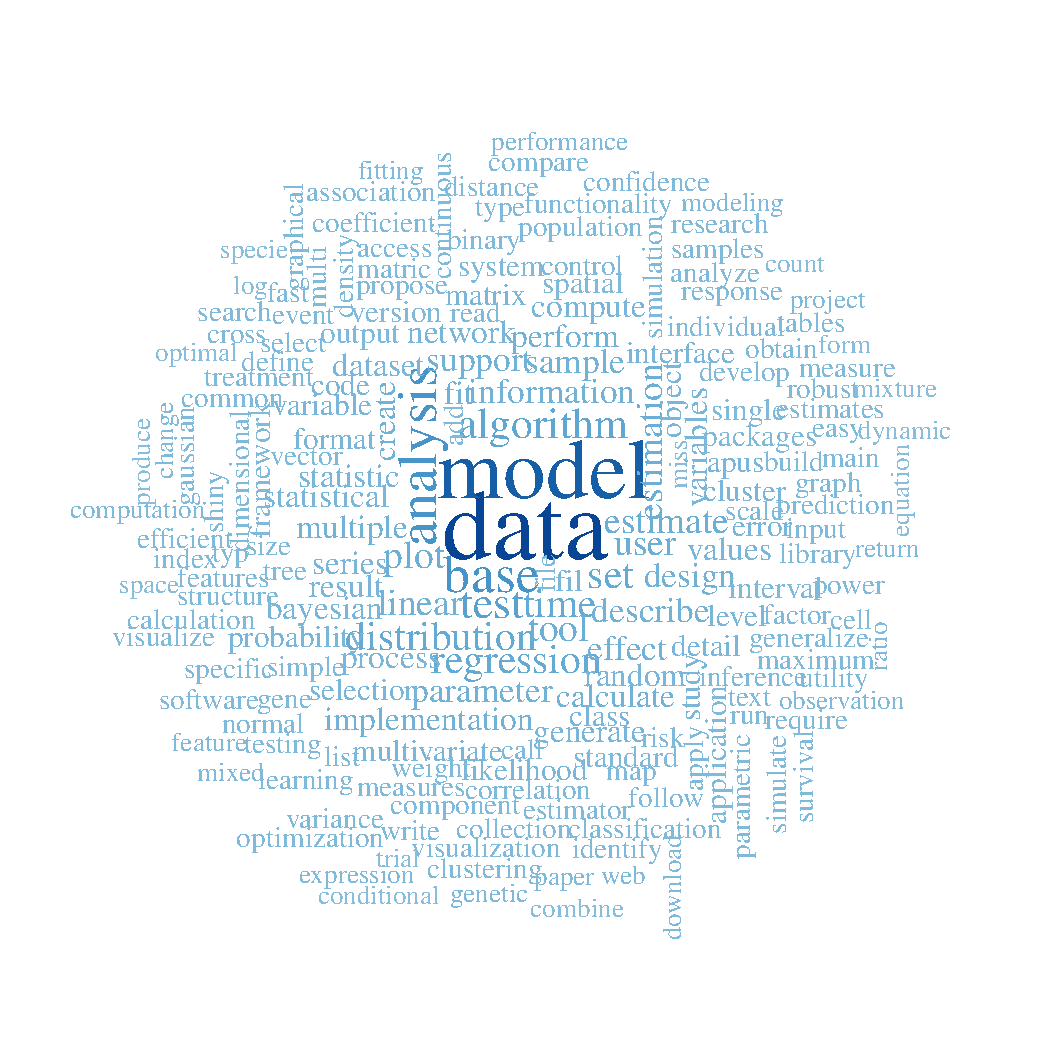
\includegraphics[width=10cm]{fig/wd_plot2.pdf}
    \caption{Word cloud of the top 200 frequently used words in the CRAN package descriptions.}
    \label{fig:wd_plot}
\end{figure}
	

\subsection{Word and Phrase Frequency}

In Figure 1, a word cloud depicts the top 200 frequently used words in the package descriptions. Each of these 200 words was used more than 400 times. Four of them appeared more than 4,000 times ({\it data, model, analysis, base}), and {\it data} is the only one appeared more than 10,000 times. These words (e.g., {\it data}, {\it model}) are related to data analysis and were also commonly used in data science curricula \citep{zhang2021data}. 



Figure~\ref{fig:freq} includes the top 30 frequently used one-, two-, and three-word phrases in the package descriptions, including phrases that are related to statistical models (e.g., {\it regression model, structural equation modeling}), estimation methods (e.g., {\it least squares, maximum likelihood estimation}), different types of datasets (e.g., {\it high dimensional data, gene expression data}), and other common and general terms in data science (e.g., {\it data analysis, variable selection, open source}). We also explored the frequently used four-word phrases, and the top phrases include {\it Markov chain Monte Carlo} (141 times), {\it genome wide association study} (51 times), {\it single cell RNA sequencing} (43 times), {\it generalized linear mixed model} (36 times), {\it cox proportional hazards model} (30 times), and {\it random effects meta analysis} (15 times). Moreover, we found two informative six-word phrases that represent the journals that were commonly mentioned in the package descriptions: {\it Journal of the American Statistical Association} (22 times) and {\it Journal of Computational and Graphical Statistics} (12 times).



\begin{figure}
\subfigure[Word]{
%\begin{minipage}[t]{0.25\linewidth}
\centering
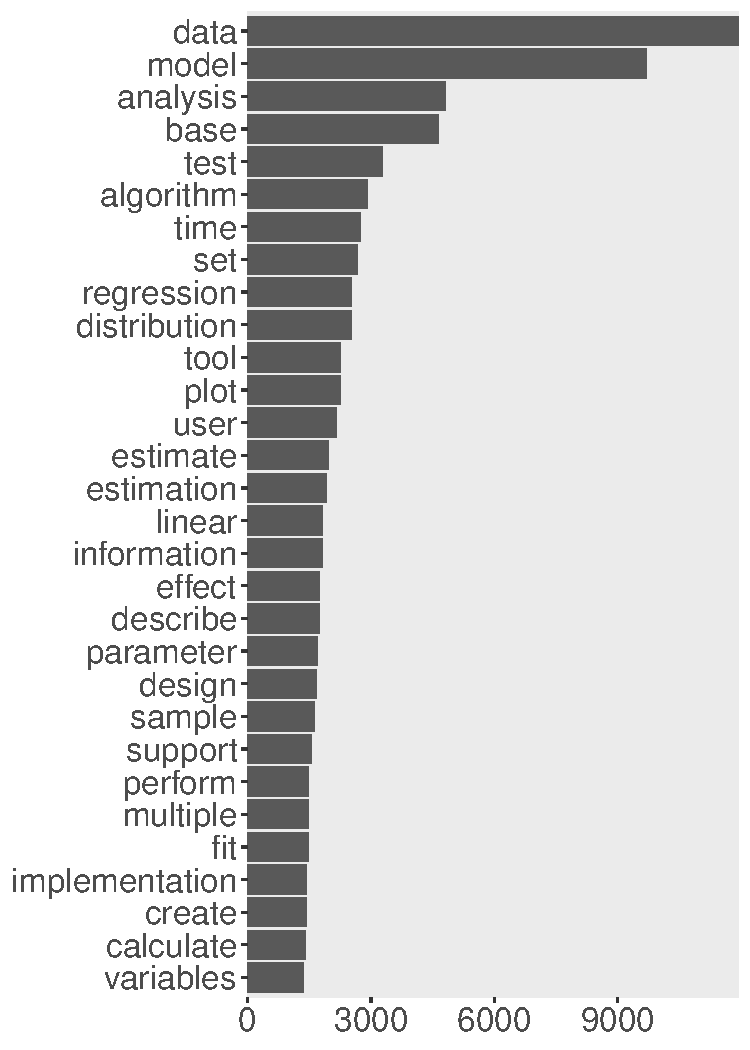
\includegraphics[width=1.8in]{fig/word1.pdf}
}%
\quad
\subfigure[Two-word phrases]{
%\begin{minipage}[t]{0.25\linewidth}
\centering
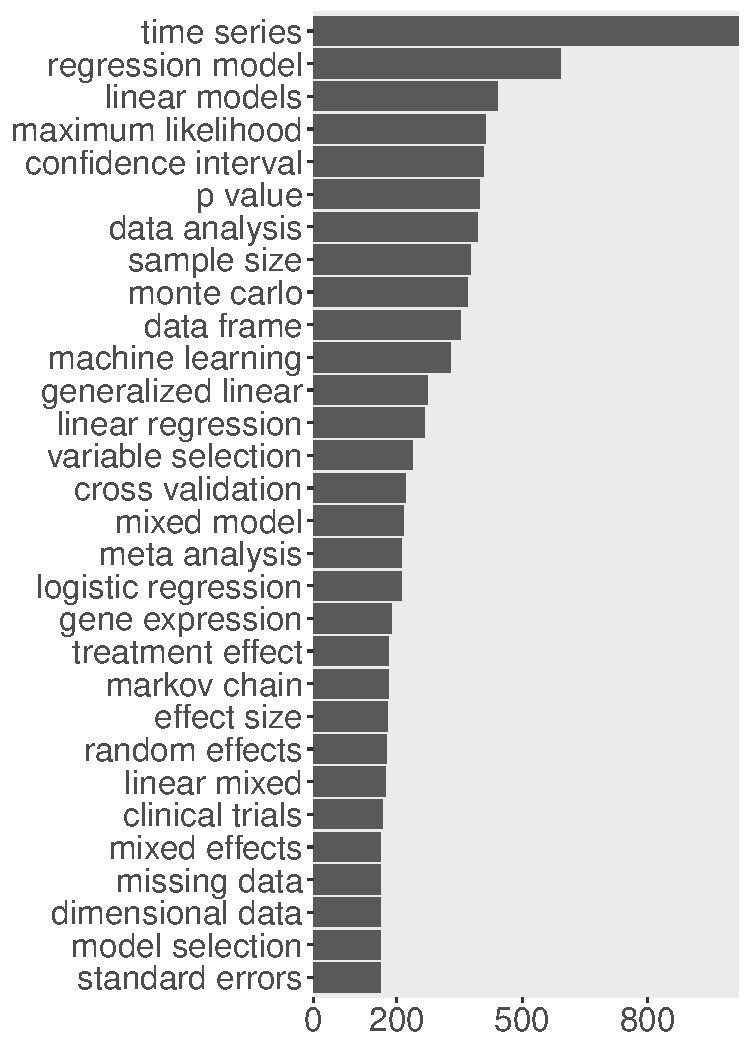
\includegraphics[width=1.8in]{fig/word2.pdf}
}%
\quad
\subfigure[Three-word phrases]{
%\begin{minipage}[t]{0.25\linewidth}
\centering
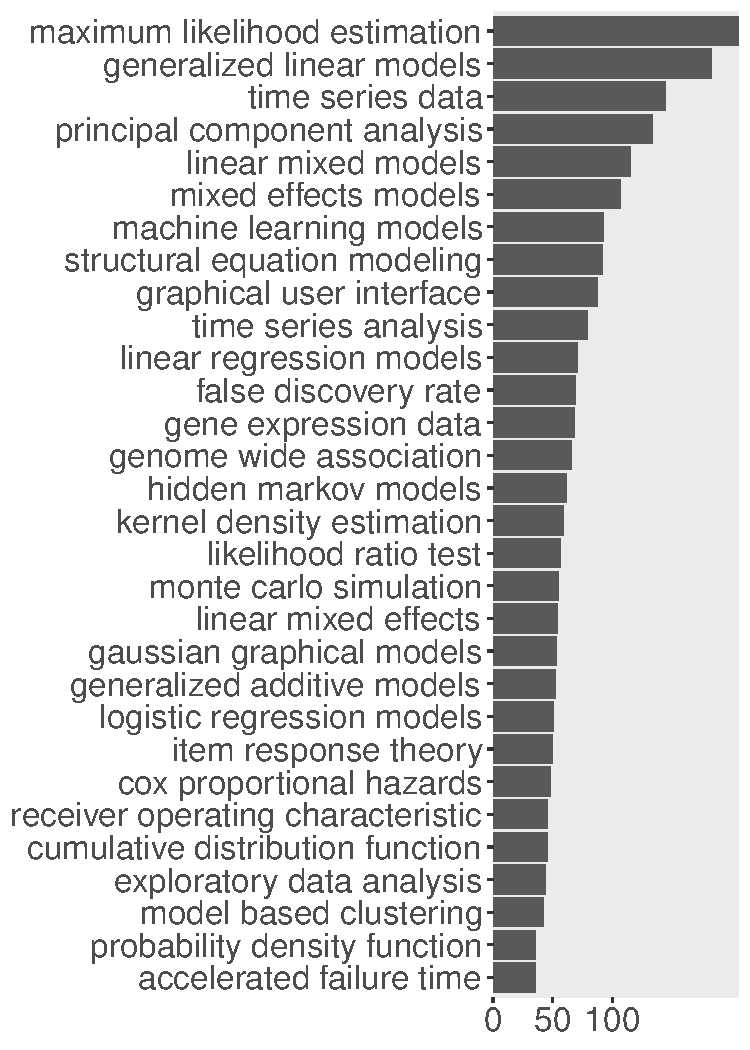
\includegraphics[width=1.8in]{fig/word3.pdf}
%\caption{fig1}
%\end{minipage}%
}


\caption{Top 30 frequently used words and phrases in the CRAN package descriptions.}

\label{fig:freq}
\end{figure}


\subsection{Topic Modeling}



To identify relevant thematic features of the CRAN R packages, we conducted topic modeling based on the package descriptions using the \CRANpkg{topicmodels} \citep{topicmodels} package. We used the Latent Dirichlet allocation (LDA; \citealp{blei2003latent}) method to reveal the latent structures in R package descriptions. LDA assumes that each document (i.e., the description document of each package) is a mixture of topics, and each topic consists of a mixture of words \citep{silge2017text}.

To fit the model, we first determined the number of topics. For each specified number of topics, ranging from 2 to 30, we built the LDA models with 100 different random number seeds to improve the robustness of results. In each replication, the 5-fold cross-validation technique was employed. We assessed the performance of the LDA models by calculating their perplexity under different numbers of topics. A low perplexity score indicates better model performance \citep{bao2014simultaneously}.  Results suggest that the best fit to the data was a model with 19 topics, followed by the 21- and 20-topic models (Figure~\ref{fig:prep_plot}). In the 100 replications of analysis, the 19-topic model was selected as the best model most frequently, followed by the 21-, 20-, 18-, and 17-topic models. By exploring the meaning of each topic in each model, we found that the model with 20 topics offered the best interpretability. The 21-topic model identified three topics which are hard to distinguish because they were all about mixed models, Bayesian analysis, linear regression, and psychometrics.  Compared to the 19-topic model, the 20-topic model was easier to interpret because it clearly separated the topics of {\it Generalized Linear Modeling and Mixed Models}, and {\it Psychometrics}. We also examined the inflection points in the performance curve (Figure~\ref{fig:prep_plot}). We found that the 9-topic and 10-topic models could not clearly differentiate many topics, resulting in many similar topics with overlapping components. Therefore, we finally adopted the 20-topic model. 


The R package \CRANpkg{ctv} (CRAN Task Views) introduces the relevant packages of 42 topics (e.g., Bayesian Inference, Chemometrics, Econometrics). We further compared the identified 20 topics with the topics classified in the CRAN Task Views and highlighted their connections in Table~\ref{tab:topic_cran}. In detail, the main topics recovered from the 20-topic LDA model, in no particular order, were listed below.


\begin{figure}[h]
\centering
    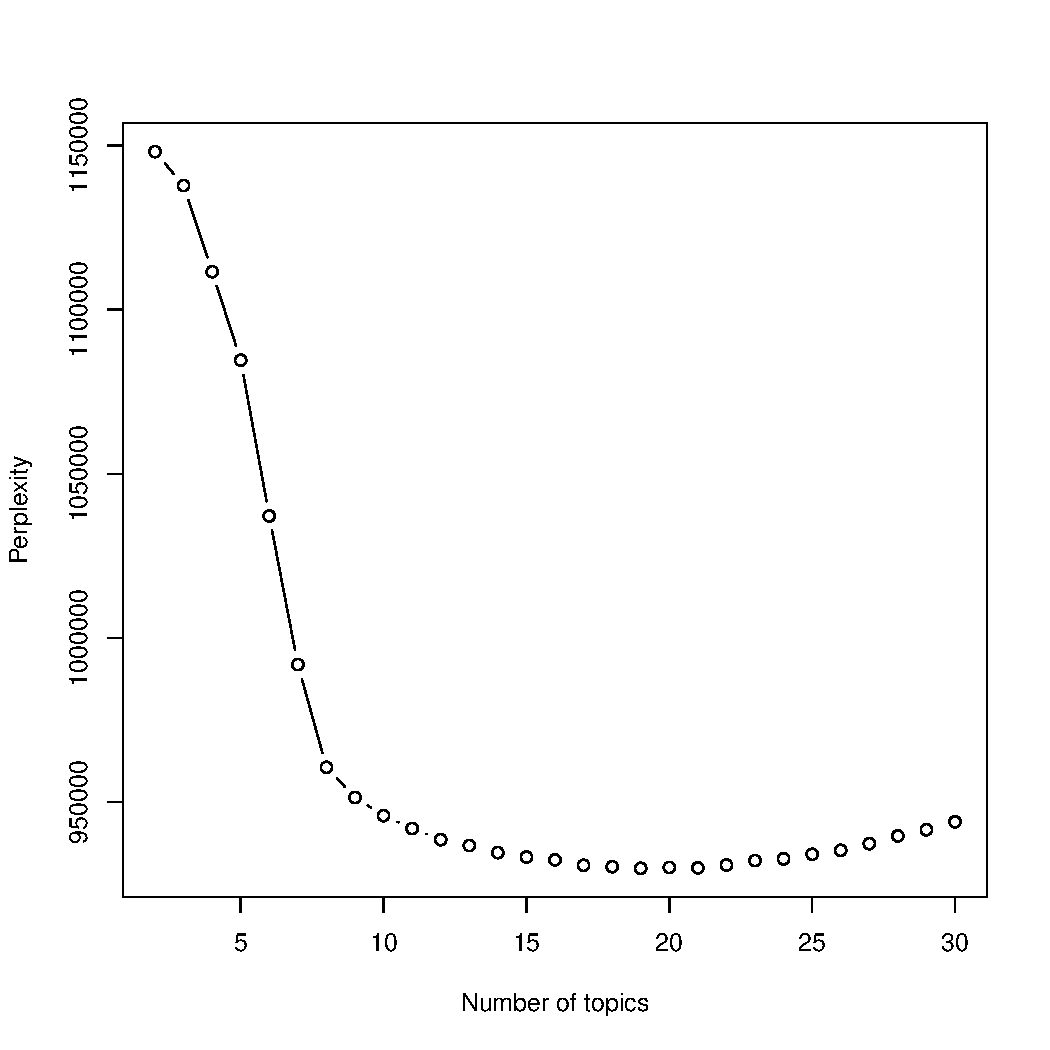
\includegraphics[width=8cm]{fig/perp_mean_plot30.pdf}
    \caption{Mean perplexities of topic models with different number of topics.}
    \label{fig:prep_plot}
\end{figure}


\begin{table}[h]
\tabcolsep 2pt \caption{Relevant CRAN Task Views of each topic identified in the topic model.} \vspace{0.0in}
\begin{center} \label{tab:topic_cran}
\resizebox{\textwidth}{!}{
\begin{tabular}{lllllll}
\toprule
Topic & CRAN Task Views \\
 \midrule
1. Supporting Packages & \href{https://cran.r-project.org/web/views/TeachingStatistics.html}{Teaching Statistics} \\
2. Causal Inference & \href{https://cran.r-project.org/web/views/CausalInference.html}{Causal Inference} \\
3. Numerical Mathematics & \href{https://CRAN.R-project.org/view=NumericalMathematics}{Numerical Mathematics} \\ 
4. Classification & \href{https://cran.r-project.org/web/views/MachineLearning.html}{Machine Learning \& Statistical Learning} \\
5. Regression Analysis and Regularization & \href{https://cran.r-project.org/web/views/MachineLearning.html}{Machine Learning \& Statistical Learning} \\
6. Genetics & \href{https://cran.r-project.org/web/views/Genetics.html}{Statistical Genetics} \\
7. Datasets & \href{https://cran.r-project.org/web/views/Databases.html}{Databases with R}  \\
8. Cluster Analysis and Network Analysis  & \href{https://cran.r-project.org/web/views/Cluster.html}{Cluster Analysis \& Finite Mixture Models}, \\ & \href{https://cran.r-project.org/web/views/gR.html}{gRaphical Models in R}  \\
9. Machine Learning & \href{https://cran.r-project.org/web/views/MachineLearning.html}{Machine Learning \& Statistical Learning} \\
10. NHST and Multiple Comparison &  - \\
11. Probability Distributions and Bayesian Analysis & \href{https://cran.r-project.org/web/views/Distributions.html}{Probability Distributions}, \\ & \href{https://cran.r-project.org/web/views/Bayesian.html}{Bayesian Inference} \\
12. Color Patterns and R Objects & - \\
13. Phylogenetics & \href{https://cran.r-project.org/web/views/Phylogenetics.html}{Phylogenetics} \\
14. Time Series Analysis & \href{https://cran.r-project.org/web/views/TimeSeries.html}{Time Series Analysis}\\
15. Data Import, Export, and Wrangling &  - \\
16. Computational Efficiency & \href{https://cran.r-project.org/web/views/Optimization.html}{Optimization and Mathematical Programming},
\\ & \href{https://cran.r-project.org/web/views/HighPerformanceComputing.html}{High-Performance and Parallel Computing with R} \\
17. Experimental Design and Clinical Trails & \href{https://cran.r-project.org/web/views/ClinicalTrials.html}{Clinical Trial Design, Monitoring, and Analysis},
\\ & \href{https://cran.r-project.org/web/views/ExperimentalDesign.html}{Design of Experiments \& Analysis of Experimental Data} \\
18. Data Visualization, Result Presentation,  & \href{https://cran.r-project.org/web/views/Graphics.html}{Graphic Displays \& Dynamic Graphics \& Graphic Devices \& Visualization},
\\ \,\,\,\,\,\,\, and Interactive Web Applications & \href{https://cran.r-project.org/web/views/ReproducibleResearch.html}{Reproducible Research} \\
& \href{https://cran.r-project.org/web/views/WebTechnologies.html}{Web Technologies and Services} \\
19. Generalized Linear Modeling and Mixed Models & \href{https://cran.r-project.org/web/views/MixedModels.html}{Mixed, Multilevel, and Hierarchical Models in R} \\
20. Psychometrics & \href{https://cran.r-project.org/web/views/Psychometrics.html}{Psychometric Models and Methods} \\
\bottomrule
\end{tabular}}
{\small
\textit{Note.} NHST = Null Hypothesis Significance Testing.
}

\end{center}
\end{table}




\paragraph{1. Supporting Packages} Keywords of this topic include {\it data, book, support, ISBN(International Standard Book Number), tool}, and {\it publication}.  This topic pertains to packages that offer supporting functions for other packages (e.g., \CRANpkg{iemisc}) and/or provide supplementary materials (e.g., datasets) for books, courses, and other packages (e.g., \CRANpkg{EnvStats}, \CRANpkg{AER}, \CRANpkg{uwo4419}, \CRANpkg{ACSWR}, \CRANpkg{mosaic}). 



\paragraph{2. Causal Inference} This topic deals with causal inference, and its keywords include {\it effect, treatment, causal, outcome, propensity}, and {\it intervention}. Packages of this topic are related to the CRAN Task View of \href{https://cran.r-project.org/web/views/CausalInference.html}{Causal Inference}. Example packages are \CRANpkg{CBPS} which contains methods for moments-based propensity score estimation, \CRANpkg{BCEE} for Bayesian Causal Effect Estimation, and \CRANpkg{CausalGAM} for estimation of causal effects with generalized additive models. 


\paragraph{3. Numerical Mathematics} Keywords of this topic include {\it matrix, sparse, covariance, correlation, vector, row, column}, and {\it decomposition}. It is related to a CRAN Task View of \href{https://cran.r-project.org/web/views/NumericalMathematics.html}{Numerical Mathematics}. Packages identified by this topic include \CRANpkg{Matrix}, a core package for sparse and dense matrix classes and methods, \CRANpkg{PRIMME}, an R interface to a C library for computing eigenvalues, \CRANpkg{SparseM}, a package with sparse linear algebra functions.


\paragraph{4. Classification} This topic is about classification and includes keywords such as {\it variable, split, random, forest, tree, category}, and {\it feature}. Example packages include \CRANpkg{randomForest} for classification based on a forest of trees, \CRANpkg{tree} containing functions for classification and regression trees, \CRANpkg{rpart} for recursive partitioning and regression trees, and \CRANpkg{C50} for fitting C5.0 classification trees and rule-based models. Some of the packages identified by this topic can be found in the CRAN Task View of \href{https://cran.r-project.org/web/views/MachineLearning.html}{Machine Learning and Statistical Learning}.

 

\paragraph{5. Regression Analysis and Regularization} This topic is about regression analysis and regularization, with words such as {\it linear, regression, model, L1, lasso, ridge, shrinkage, procedure}, and {\it regularization} appearing with high probability. It is related to the packages for regularization methods and regression models (e.g., \CRANpkg{glmnet} for lasso and elastic-net regularized generalized linear models (GLMs), \CRANpkg{penalized} for applying ridge and lasso regularization in GLMs and Cox proportional hazards models, and \CRANpkg{bravo} for Bayesian variable selection with ultra-high dimensional linear regression models.). 



\paragraph{6. Genetics} Keywords of this topic include terms related to genetics, such as {\it gene, RNA (Ribonucleic Acid), DNA (DeoxyriboNucleic Acid), sequence, cell}, and {\it phenotype}. This topic identifies the packages for analyzing biological data, especially genetic data (e.g., \CRANpkg{jetset}, \CRANpkg{Seurat}, \CRANpkg{scBio}). 

\paragraph{7. Datasets} High probability words of this topic include {\it data, survey, questionnaire, sample, collection, census}, and {\it report}. This topic is mainly about a special kind of packages for providing datasets (especially survey data) instead of functions for statistical methods. For example, \pkg{spiR} is for social progress index data, \CRANpkg{PakPMICS2018} is for survey data of a specific project conducted from 2017 to 2018, \CRANpkg{USpopcenters} is about united stats centers of population data. 

\paragraph{8. Cluster Analysis and Network Analysis} Keywords of this topic are related to two sub-topics. First, {\it network, gaussian, graphical, node, edge}, and {\it igraph} are commonly used in network analysis. Example packages include \CRANpkg{igraph} and \CRANpkg{sna}. Second, {\it cluster, class, kernel} are relevant to Cluster Analysis. Example packages include \CRANpkg{cluster}, \CRANpkg{kml} for implementing k-means clustering on longitudinal data, \CRANpkg{flexclust} for providing flexible cluster algorithms. Cluster analysis and network analysis were identified in one topic perhaps because there are some packages for clustering based on correlation matrices and network modeling (e.g., \CRANpkg{DirectedClustering}, \CRANpkg{linkcomm}, \CRANpkg{clusterGeneration}).




\paragraph{9. Machine Learning} With keywords such as {\it algorithm, machine, learning, training}, and {\it prediction}, this topic is mainly about machine learning. The CRAN Task View of \href{https://cran.r-project.org/web/views/MachineLearning.html}{Machine Learning and Statistical Learning} lists and classifies the packages of this topic, for example, packages for neural networks, deep learning (e.g., \CRANpkg{RcppDL}, \CRANpkg{deepnet}).  Some packages are related to both this topic and the topic of regularization (e.g., \pkg{bmrm}). Courses of this topic are also very common in data science programs, including {\it Neural Networks and Deep Learning}, and {\it Machine Learning and Big Data} \citep{zhang2021data}.

\paragraph{10. Null Hypothesis Significance Testing (NHST) and Multiple Comparison} This topic encompasses NHST and Multiple Comparison, and its keywords include {\it test, hypothesis, null, multiple, comparison}, and {\it significance}. Relevant packages include \CRANpkg{onewaytests} for NHST, \CRANpkg{PMCMRplus} and \CRANpkg{conover.test} for multiple comparisons among multiple groups.

\paragraph{11. Probability Distributions and Bayesian Analysis} This topic centers around the word {\it distribution} and includes other relevant terms such as {\it probability, binomial, poisson, density, Bayesian, MCMC (Markov chain Monte Carlo), chain, prior, posterior}, and {\it sampler}. Probability and Bayesian analysis were identified in one topic because they share the main keyword {\it distribution} (i.e., probability distribution, prior distribution, and posterior distribution). Example packages include \CRANpkg{extraDistr} for various univariate and multivariate distributions, \CRANpkg{gnorm} for generalized normal or exponential power distributions, \CRANpkg{bayesmix} for Bayesian mixture models, and \CRANpkg{mcmc}. The CRAN Task Views of \href{https://cran.r-project.org/web/views/Distributions.html}{Probability Distributions} and \href{https://cran.r-project.org/web/views/Bayesian.html}{Bayesian} provided a detailed summary of packages related to this topic.


\paragraph{12. Color Patterns and R Objects} Keyword of this topic include {\it class, object, s4}, and{\it r6} which are related to R objects, and {\it color, png, image}, and {\it palettes} which are about visualization. For the R objects, example packages are \CRANpkg{R6}, \CRANpkg{R62S3}, and \CRANpkg{fastdigest}. For the visualization, most packages identified by this topic are designed to provide color patters for plotting (e.g., \CRANpkg{colormap}, \CRANpkg{ggpattern}). Package \CRANpkg{ggplot2} is also identified by this topic, but its relationship with the topic 18 (Data Visualization, Result Presentation, and Interactive Web Applications) is higher than its relationship with this topic.


\paragraph{13. Phylogenetics} This topic is mainly about phylogenetics, with high probability words including {\it phylogenetic, specie, signal, taxonomic, animal, pedigree}, and {\it biodiversity}. Packages related to this topic include \CRANpkg{phytools} which provides functions for phylogenetic analysis, \CRANpkg{geiger} for fitting macroevolutionary models to phylogenetic trees, and \CRANpkg{phylosignal} for exploring the phylogenetic signal. The CRAN Task View \href{https://cran.r-project.org/web/views/Phylogenetics.html}{Phylogenetics} also summarized packages related to this topic.



\paragraph{14. Time Series Analysis} This topic is mainly about time series analysis. The high probability words associated with this topic include {\it time, series, change, dynamic, forecast, growth, trend}, and {\it lag}. There is a CRAN Task View of this topic that introduces many packages for handling time series data, for example, \CRANpkg{tseries} for time series analysis, and \CRANpkg{forecast} that provides forecasting functions for time series models.


\paragraph{15. Data Import, Export, and Wrangling}  This topic includes keywords such as {\it read, load, import, write, convert}, and {\it create}, which are commonly-used verbs for naming R functions for data import, export and wrangling. Example packages include \CRANpkg{asciiSetupReader}, which can read fixed-width ASCII data files, \CRANpkg{adfExplorer}, which can import and export Amiga disk files, and \CRANpkg{dplyr}, "a grammar of data manipulation."

\paragraph{16. Computational Efficiency} This topic is related to computational efficiency, with keywords including {\it run, C++, fast, efficient, Rcpp, efficient}, and {\it parallel}. Many packages associated with this topic call compiled C++ code from R to improve performance (e.g., \CRANpkg{Rcpp}), and provide utilities for parallel computation (e.g., \CRANpkg{future.callr}, \CRANpkg{foreach}, \CRANpkg{doParallel}).

\paragraph{17. Experimental Design and Clinical Trails} This topic focuses on the design and data analysis of experiments and clinical trials. High probability words include {\it design, treatment, control, trial, clinical, sample, size, endpoint, stage, dose}, and {\it experimental}. The CRAN Task Views of \href{https://cran.r-project.org/web/views/ClinicalTrials.html}{Clinical Trial Design} and \href{https://cran.r-project.org/web/views/ExperimentalDesign.html}{Experimental Design} summarize two lists of R packages concerning this topic. Here we listed some example packages such as \CRANpkg{TrialSize} for sample size determination in clinical research, and \pkg{visit} for phase I dose-escalation study design.

\paragraph{18. Data Visualization, Result Presentation, and Interactive Web Applications} Packages and keywords of this topic can be classified into three sub-topics. First, keywords such as {\it ggplot2, color, graph, image}, and {\it plot} are related to data visualization. Example packages include \CRANpkg{ggplot2} and \CRANpkg{lattice}.  The second sub-topic is about presenting results, with keywords such as {\it table, chart}, and {\it figure}. Other keywords include {\it format, html, document, markdown, rmarkdown}, and {\it latex} which are mainly about R markdown tools for generating dynamic reports. Example packages are R markdown-related tools including \CRANpkg{knitr} and \CRANpkg{bookdown}, and formatting tools such as \CRANpkg{styler} and \CRANpkg{pander}. The third sub-topic relates to using R to build interactive web applications. Words relevant to this sub-topic include {\it shiny, widget, web}, and {\it XML}, and example packages include \CRANpkg{shiny} and \CRANpkg{webshot}.

In addition, there are many packages related to more than one sub-topic. For example, \CRANpkg{ANOVAShiny} was built based on \CRANpkg{rmarkdown} and \CRANpkg{shiny}, and \CRANpkg{Factoshiny} was developed with \CRANpkg{shiny} and \CRANpkg{ggplot2} for conducting factorial analysis and drawing graphs with a shiny application. There are also corresponding lists of this topic on CRAN Task Views, and courses in data science programs (e.g., {\it Data Visualization}, {\it Data Presentation and Visualization with R}; \citealp{zhang2021data}). 

\paragraph{19. Generalized Linear Models and Mixed Models} This topic is related to generalized linear modeling, with keywords such as {\it model, regression, linear, fit, mixed, logistic}, and {\it GLM (Generalized Linear Modeling)}. Packages associated with this topic include \CRANpkg{dglm} for building double generalized linear models, \CRANpkg{brms} for Bayesian Regression Models, \CRANpkg{nlme} for linear mixed models (LMMs), and \CRANpkg{mbest} for large nested LMMs.

\paragraph{20. Psychometrics} The high probability words related to this topic include {\it factor, item, response, latent, IRT (Item Response Theory)}, and {\it choice}. There is a detailed list on the CRAN Task Views about this topic. Here we listed some example packages: \CRANpkg{mirt} for multidimensional item response theory, \CRANpkg{difR} for detecting differential item functioning, and \CRANpkg{CDM} for cognitive diagnosis models.























\section{Identifying Key Packages and Key Package Developers}




To investigate the key packages contributing to the R ecosystem and the notable authors who significantly support the R community, we conducted network analysis. We extracted package dependency and authorship information from CRAN and used \CRANpkg{cranly} \citep{cranly} and  \CRANpkg{igraph}  \citep{csardi2006igraph} to build three networks: 1) a package dependency network, 2) an author collaboration network, and 3) a bipartite network of packages and authors. Influential nodes were identified in these three networks. We first introduce the one-mode network (i.e., network with one type of node) of packages and authors below.

The R package dependency network was built based on the CRAN R packages and their dependent packages, including the base and recommended R packages that are included in the default installation of R. It is a directed and weighted network, and a sub-graph is presented in Figure~\ref{fig:networka}. Specifically, the arrow from package A to package B indicates that A depends on, imports, suggests, link to, or is enhanced by B. Table~\ref{tab:connections} presents the detailed definitions and frequencies of these relationships \citep{R}. We assigned the weights of edges as $5, 4, 3, 2,$ and $1$ for the relationships of {\it depends, imports, suggests, links to}, and {\it enhances}, respectively.

We tested a different weight scheme $(3, 2, 1, 1, 1)$ and found that the results were robust, with correlations of influence scores exceeding .95. The top packages identified were also similar. Hence, we report results based on the $(5, 4, 3, 2, 1)$ weight scheme in this paper.

For the undirected author collaboration network (e.g., Figure~\ref{fig:networkb}), the edge between two nodes indicates that they have co-authored in at least one package. The weights of edges denote the number of packages co-authored by the corresponding two authors.




\begin{table}[h]
\tabcolsep 2pt \caption{Types of Package Dependencies.} \vspace{0.0in}
\begin{center} \label{tab:connections}
\begin{tabular}{lllllll}
\toprule
Dependency & Definition & Frequency\\
 \midrule
Depends & B will be attached when attaching A  & 10523 \\
Imports & The namespace of B will be imported when attaching A & 87328\\ % but B will not be attached
Suggests & B is used on in the examples, tests, or vignettes of A & 54991\\
Links to & A uses the header files in B to compile its C or C++ code & 5153\\
Enhances & B provides methods for classes in A, or helps handling objects in A & 558\\
\bottomrule
\end{tabular}
\end{center}
\end{table}



\begin{figure}
\begin{center}

\subfigure[Fifteen packages with the highest in-degrees]{
%\begin{minipage}[t]{0.25\linewidth}
\centering
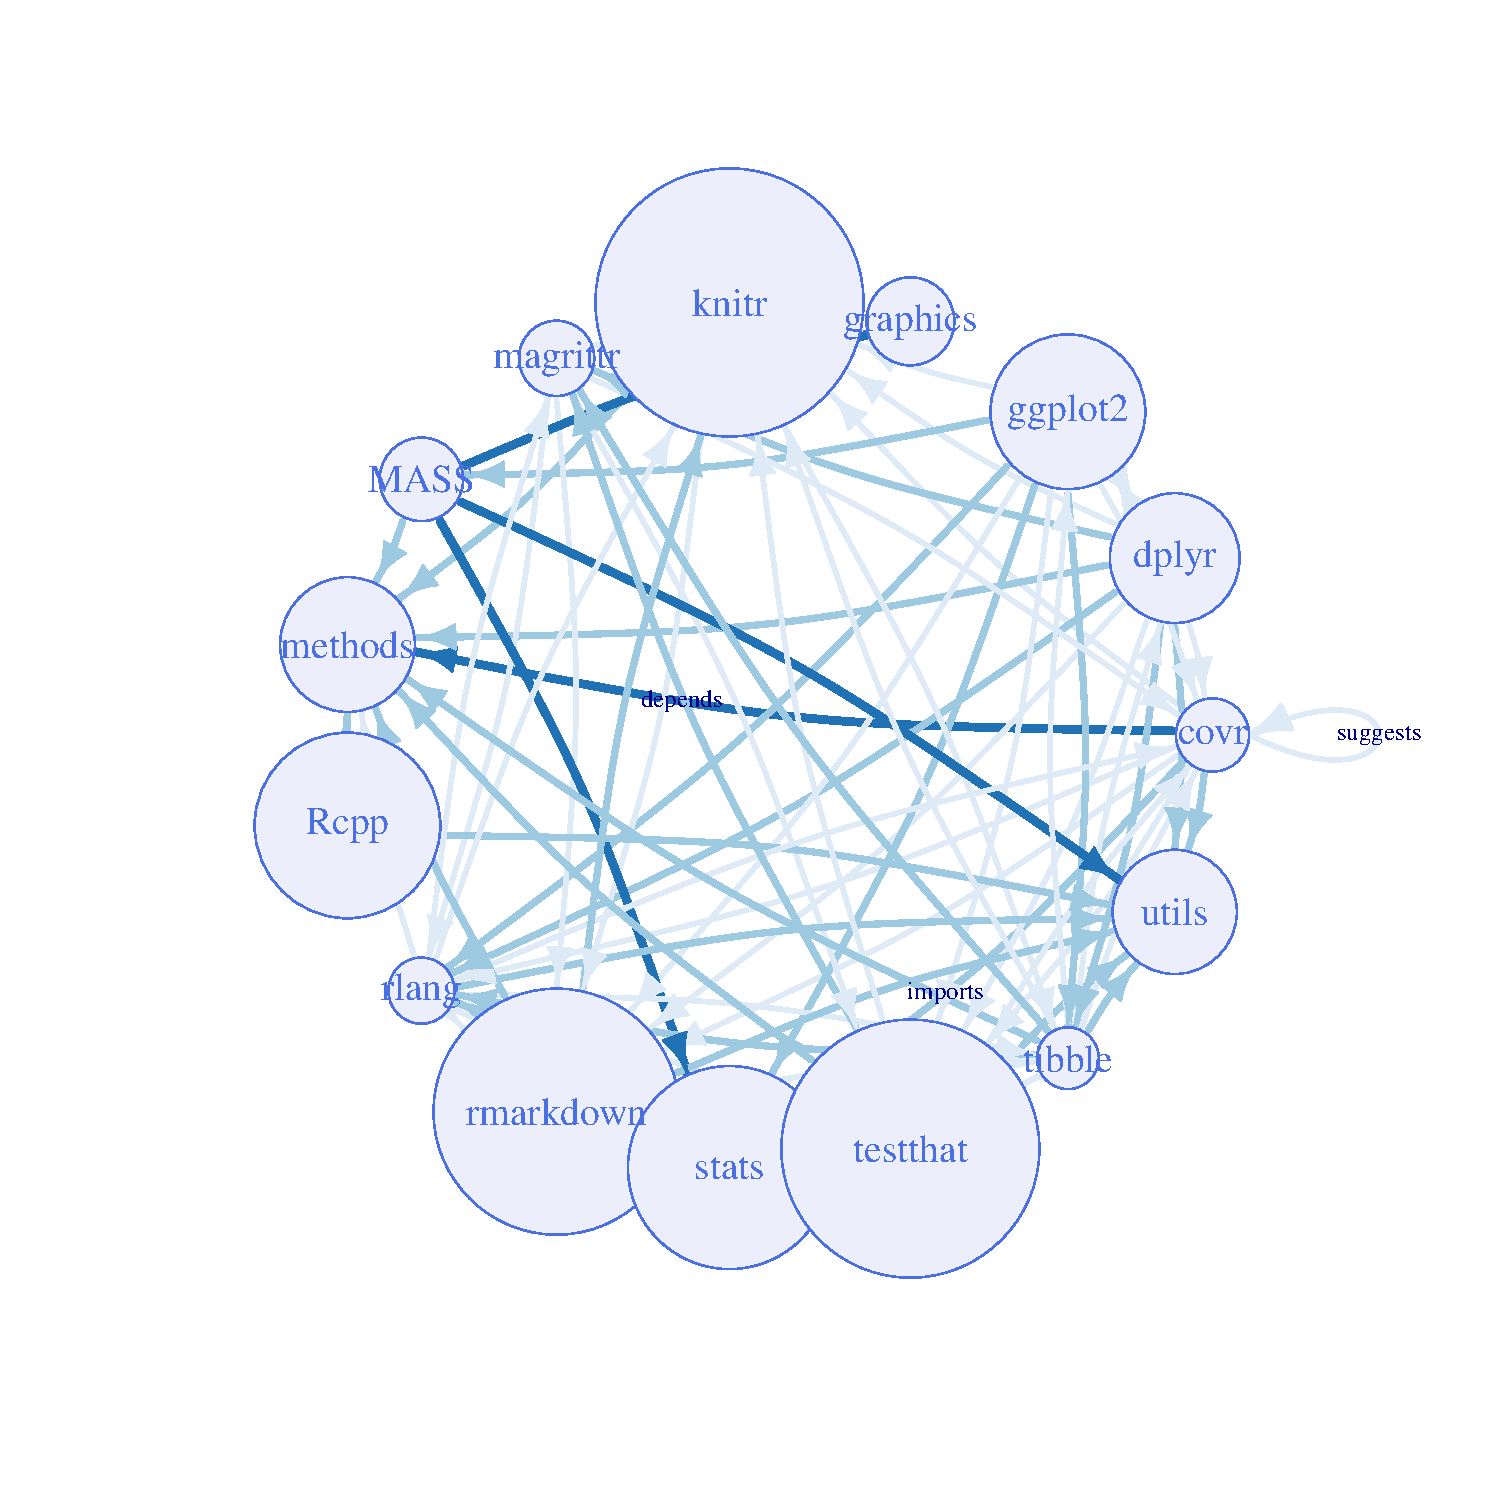
\includegraphics[width=2.7in,trim=35 35 35 35,clip]{fig/plot_pkg.pdf}
\label{fig:networka}
%\caption{fig1}
%\end{minipage}%
}%
\quad
\subfigure[Fifteen authors with the highest degrees]{
%\begin{minipage}[t]{0.25\linewidth}
\centering
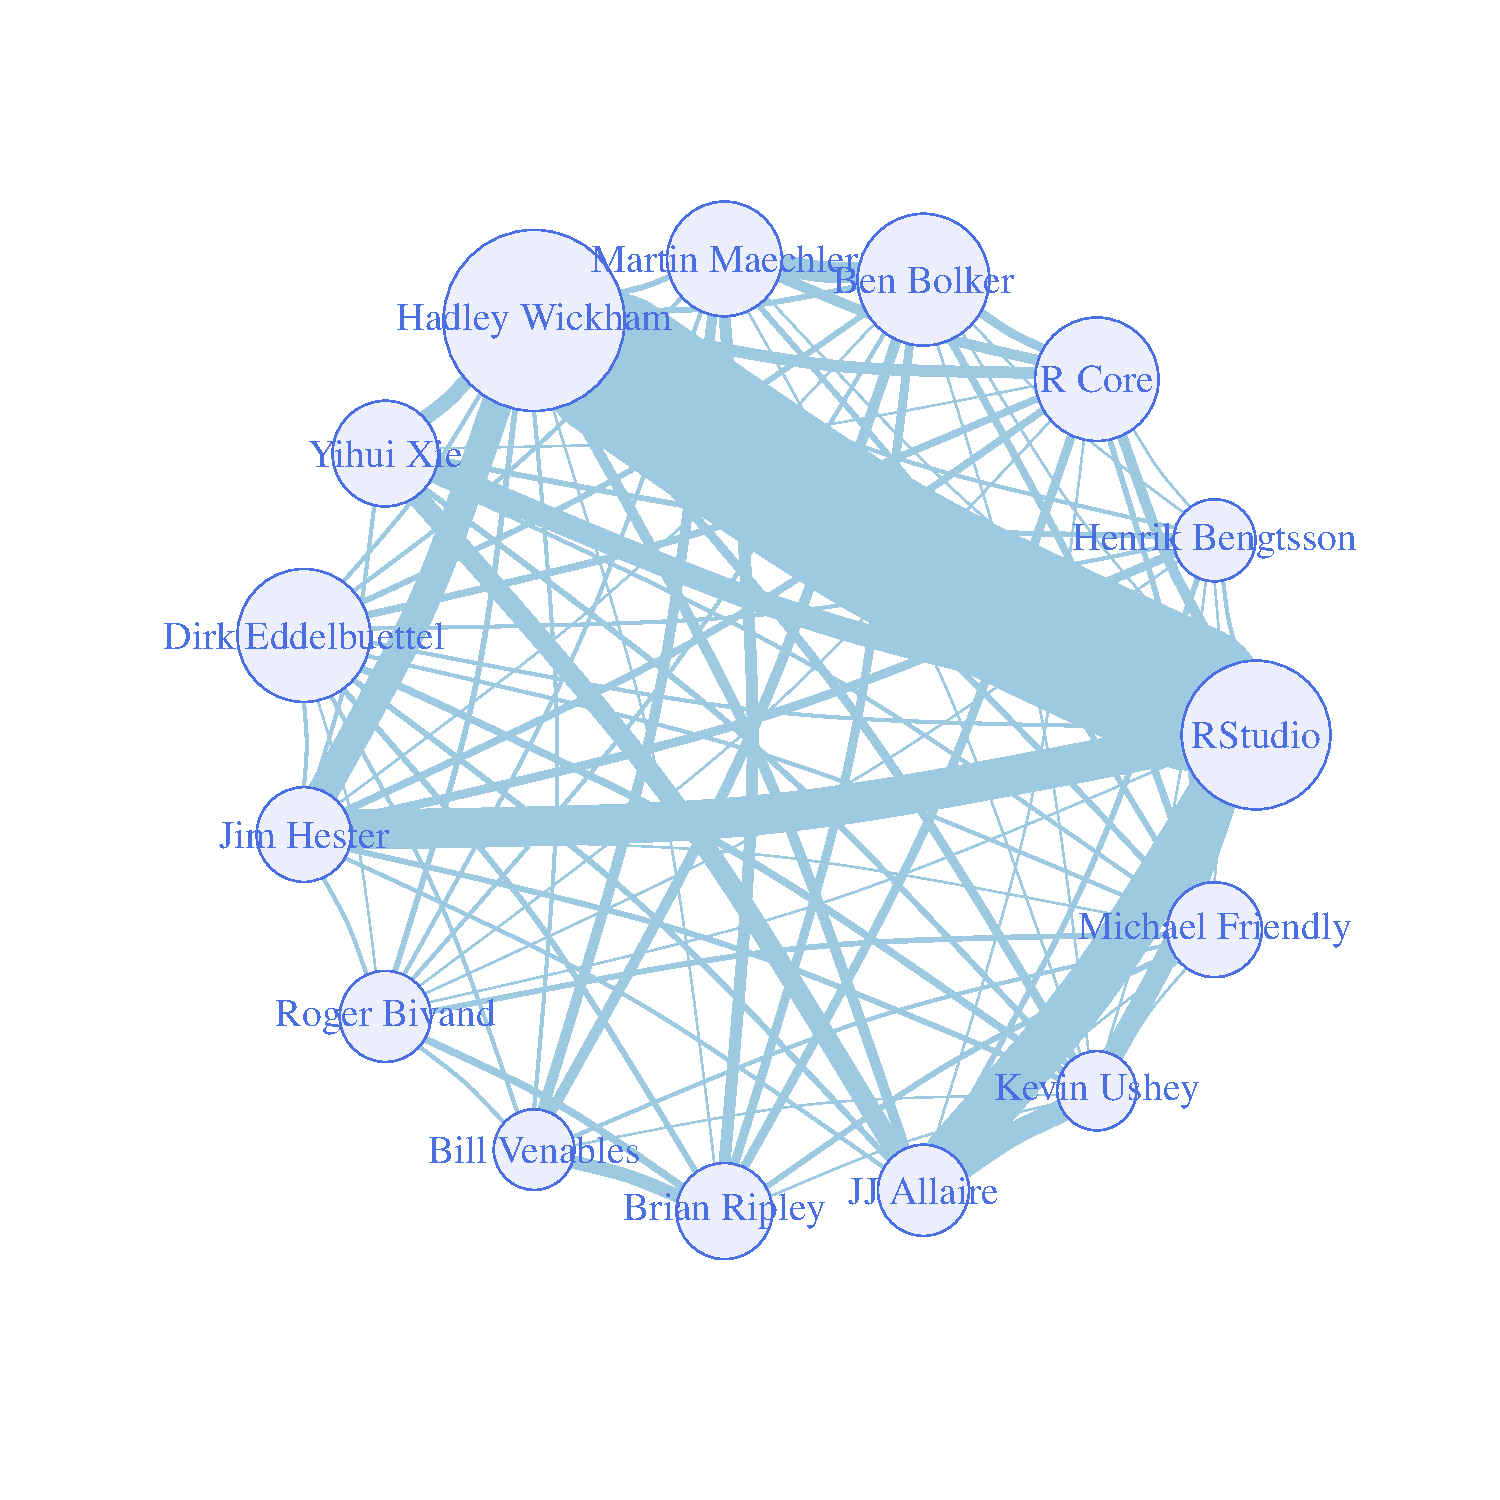
\includegraphics[width=2.5in,trim=50 50 50 50,clip]{fig/plot_aut.pdf}
\label{fig:networkb}
%\caption{fig1}
%\end{minipage}%
}%
\caption{Networks of a subset of nodes with the highest degrees.}
\end{center}

{\small
\textit{Note.} The sizes of nodes represent the in-degree / degree of nodes. In the author collaboration network, the edge width reflects the weight. In the package dependency network, the color indicates the weight. "The dark edges represent {\it depends}, medium dark edges represent {\it imports}, the lightest edges represent {\it suggests}. Relationships of {\it linking to} and {\it enhances} are not included in this sub-graph.
}

\end{figure}





\subsection{Measures of Influence}

We focused on the following commonly used measures for evaluating node (a package or an author) influence in the one-mode network (\citealp{jain2020identification}; \citealp{morone2015influence}; \citealp{salavaty2020integrated}; \citealp{wang2017ranking}): 

\begin{itemize}
	\item Local structure information: Degree;
	\item Global structure information: Betweenness \citep{freeman1978centrality};
	\item Algorithm based on random walk: Eigenvector centrality \citep{bonacich1972factoring} and PageRank \citep{page1999pagerank};
\end{itemize}
%Detailed definition of each index was summarized below.

\paragraph{Degree and In-degree}

Degree is the number of direct connections between nodes. For the directed package dependency network, in-degree indicates how many packages this package enhances, or is depended on, imported, suggested, or linked by.  For the undirected author collaboration network, degree is the number of collaborators.

\paragraph{Betweenness Centrality}

Betweenness quantifies how important a node is as a mediator between two other nodes. Given a network, the betweenness centrality of node $i$ can be calculated as \citep{freeman1978centrality}:

\begin{equation}
C_{Bet}(i)= \sum_{s\neq i \neq t} \frac{d_{s,t}(i)}{d_{s,t}}
\end{equation}
where $d_{s,t}$ denotes the number of shortest paths from node $s$ to node $t$, and $d_{s,t}(i)$ is the number of shortest paths between node $s$ and node $t$ going through node $i$. %Note that weights were not considered in calculating the betweenness centrality. This is because, in the \CRANpkg{igraph} package, weights are viewed as distances for calculating the betweenness, which is not consistent with the current study. 



\paragraph{Eigenvector Centrality}

A node with a small degree may have high eigenvector centrality \citep{bonacich1972factoring} if it is connected with important nodes. In other words, this index considers the importance of neighbors when evaluating the centrality of a node.

Let $A = (a_{i,j})$ be the adjacency matrix of a graph, where $a_{i,j}$ represents the connection between node $i$ and $j$. The eigenvector centrality of node $i$ is given by \citep{bonacich2007some}:

\begin{equation}
C_{Eig}(i)= \frac{1}{\lambda} \sum_j a_{i,j} \, C_{Eig}(j)
\end{equation}
where $\lambda$ is a non-zero eigenvalue. This can also be expressed in the matrix form:

\begin{equation}
\lambda C_{Eig} = C_{Eig} A
\end{equation}
where $C_{Eig}$ is the eigenvector for the adjacency matrix $A$ given eigenvalue $\lambda$. \citet{bonacich1972factoring} suggested to choose the largest value of $\lambda$ for measuring centralities. % this choice guarantees the following desirable property: if matrix $A$ is irreducible, or equivalently if the graph is (strongly) connected, then the eigenvector solution $x$ is both unique and positive.
%https://www.sci.unich.it/~francesc/teaching/network/eigenvector.html




\paragraph{PageRank}

PageRank is a variant of eigenvector centrality. It is an algorithm developed by Google to rank web pages \citep{page1999pagerank}, and is primarily used for directed networks. Given a weighted network, it can be calculated as:
\begin{equation}
%PR(i)= k \sum_j a_{i,j} \frac{PR(j)}{C_{Out}(j)} + 1-k
PR(i)= \alpha \sum_j W_{j,i}PR(j) + (1-\alpha)PR^0(i)
\end{equation}
where $PR(i)$ and $PR(j)$ are the PageRank of node $i$ and $j$, respectively. Besides, $PR^0(i)$ is typically set as $\frac{1}{N}$ where $N$ is the number of nodes, $\alpha$ is the damping factor assigned to the random walk, and $W_{j,i}$ is the normalized edge weight from node $j$ to $i$:
\begin{equation}
W_{j,i} = \frac{w_{j,i}}{\sum_t w_{j,t}}
\end{equation}
where $w_{j,i}$ is the edge weight from node $j$ to node $i$. 
%https://github.com/igraph/igraph/issues/1211





\subsection{Bipartite Network}

A bipartite network of authors and packages was built using the authorship information. The weight of an edge was assigned as 3 if the author is the maintainer of the package, and 1 otherwise (Figure~\ref{fig:bipar}). Unlike the one-mode networks, which focus on either packages or authors, the bipartite network captures both the relationships between authors and packages and the collaborations among authors. As shown in Figure~\ref{fig:net_illu}, the same author relationship configuration could be represented by two different bipartite networks. Therefore, we employed the bipartite network to gain more insights into the influential authors using the BiRank statistic.

\begin{figure}[h]
    \begin{center}   
    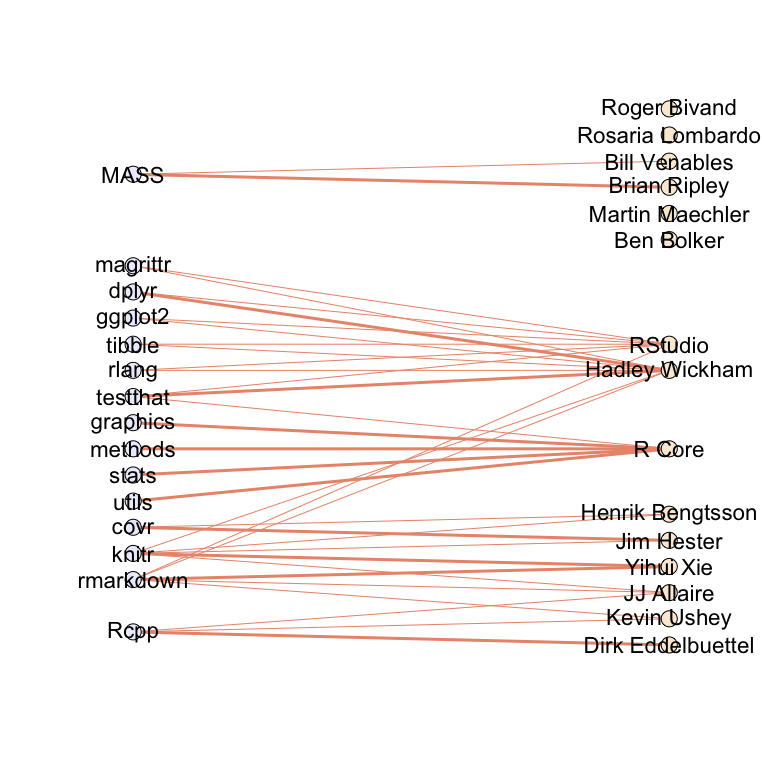
\includegraphics[width=11cm,trim=50 70 0 50,clip]{fig/plot_bipar.png}
    \caption{A Bipartite network of selected R packages and authors.} \label{fig:bipar}
    \end{center}
   {\small
\textit{Note.} Nodes on the left are 15 packages with the highest in-degrees in the package dependency network, nodes on the right are 15 authors with the highest degrees in the author collaboration network. A bold line indicates that the corresponding author is the maintainer of the corresponding package.
}


\end{figure}



\paragraph{BiRank}
\citet{aronson2020comparing} compared different centrality measures for the bipartite network and recommended the BiRank and CoHITS indexes. For our network, the BiRank index exhibited a high correlation with the CoHITS index ($r=.860$). The top 50 authors identified by these two measures are the same, with only minor variations in their ranking. Consequently, we only reported the results of the BiRank index \citep{he2016birank}.  Similar to PageRank, the BiRank index assumes that the ranking of nodes should be related to the ranking of the neighbors. Namely, an author would be ranked high if his or her neighbor packages are important.


Let $A = (a_{i,j})$ be the adjacency matrix of a bipartite graph with two types of nodes $u_i (i = 1, \ldots, I)$ and $p_j (j = 1, \ldots, J)$, the BiRank value for node $u_i$ is given by:
\begin{equation}
BR(u_i) = \alpha \sum_{j}a_{i,j}\frac{BR(p_j)}{\sqrt{C_{wDeg}(u_i)} \sqrt{C_{wDeg}(p_j)}} + (1-\alpha)BR^0(u_i)
\end{equation}
where $C_{wDeg}(u_i)$ and $C_{wDeg}(p_j)$ are the weighted degrees of node $u_i$ and $p_j$. %, they are included to reduce the dependence of BiRank values on the degree centrality.
Similar to the PageRank index, $\alpha$ is the damping factor, and $BR^0(u_i)$ is the prior belief of the importance of node $u_i$. 




\begin{figure}[h]
\centering

\subfigure[Bipartite sub-graph of one package and three authors]{
%\begin{minipage}[t]{0.25\linewidth}
\centering
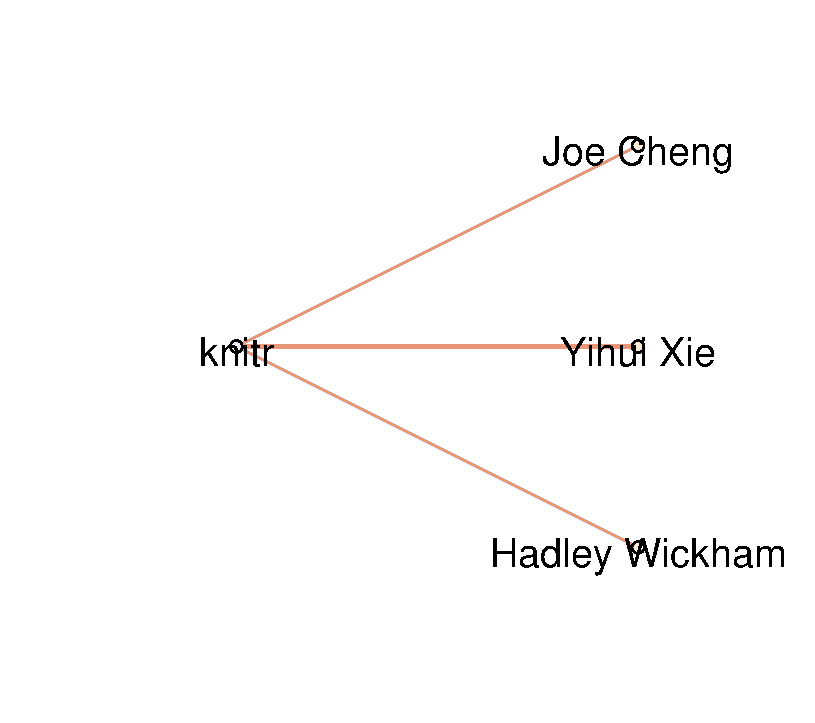
\includegraphics[width=2.5in,trim=50 70 0 50,clip]{fig/plot_bipar_illu1.pdf}
%\caption{fig1}
%\end{minipage}%
}%
\subfigure[Author collaboration network based on (a)]{
%\begin{minipage}[t]{0.25\linewidth}
\centering
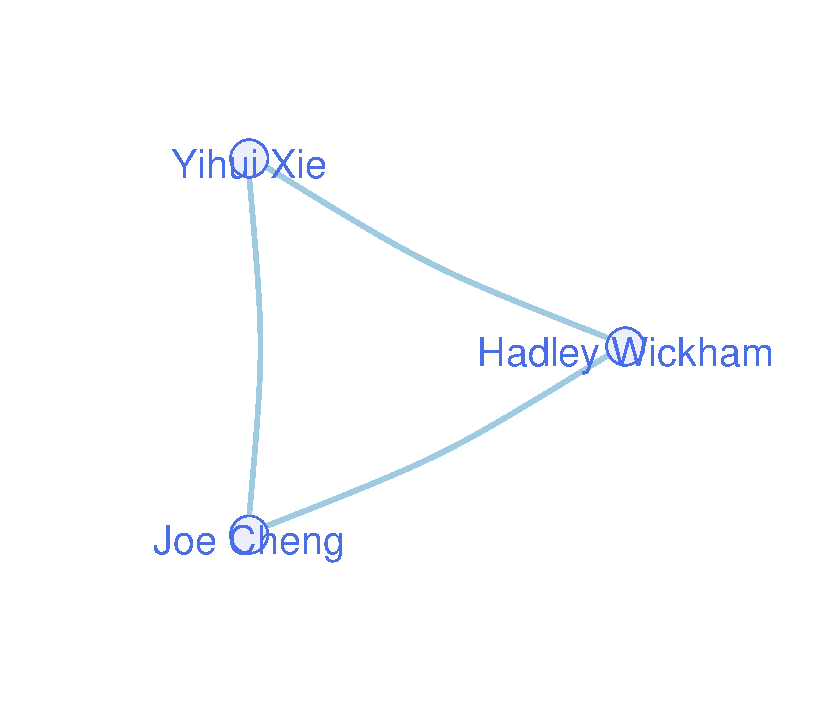
\includegraphics[width=2.5in,trim=50 70 0 50,clip]{fig/plot_aut_illu1.pdf}
%\caption{fig1}
%\end{minipage}%
}%
\quad
\subfigure[Bipartite sub-graph of three packages and authors]{
%\begin{minipage}[t]{0.25\linewidth}
\centering
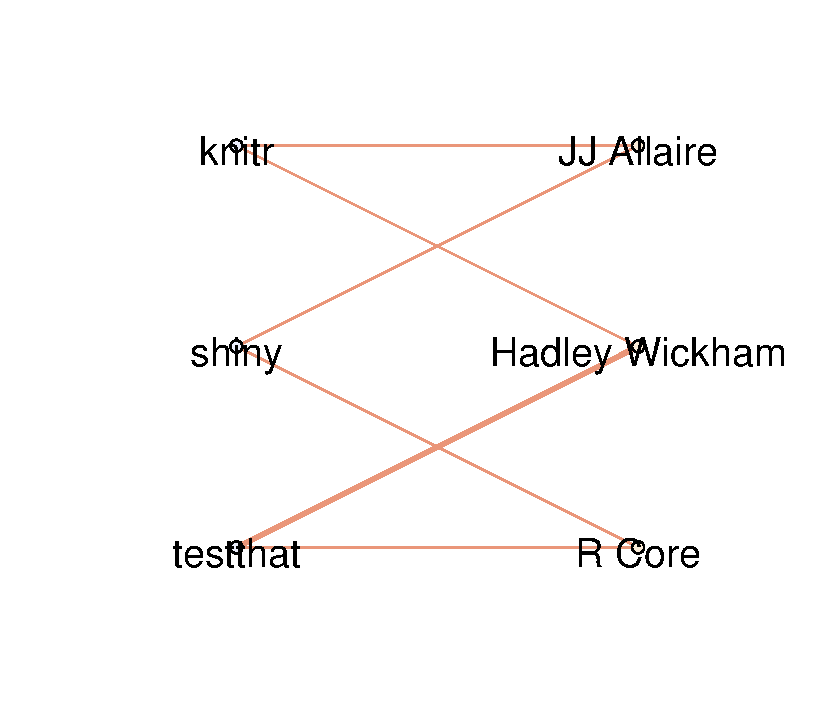
\includegraphics[width=2.5in,trim=50 70 0 50,clip]{fig/plot_bipar_illu2.pdf}
%\caption{fig1}
%\end{minipage}%
}%
\subfigure[Author collaboration network based on (c)]{
%\begin{minipage}[t]{0.25\linewidth}
\centering
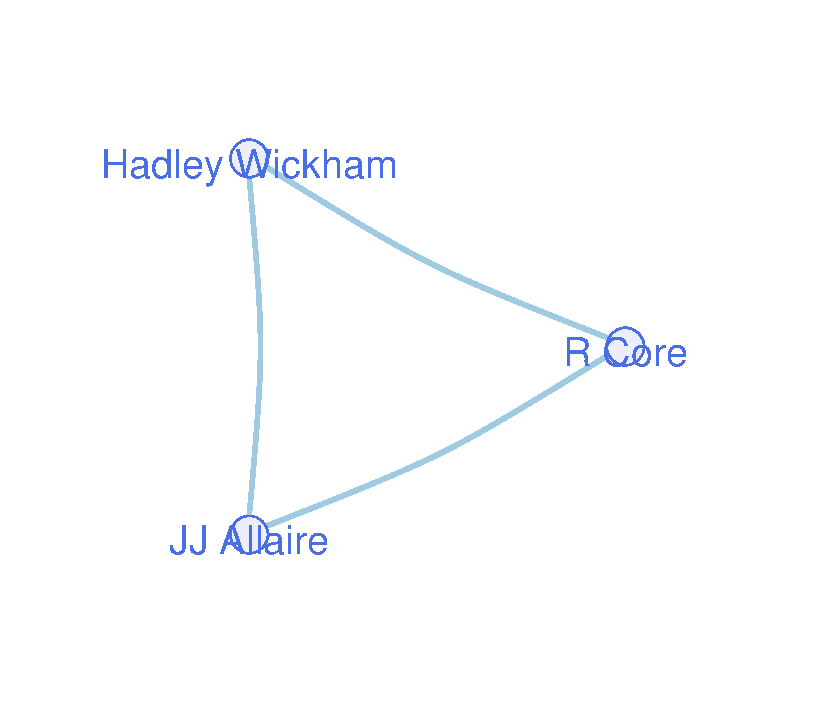
\includegraphics[width=2.5in,trim=50 70 0 50,clip]{fig/plot_aut_illu2.pdf}
%\caption{fig1}
%\end{minipage}%
}%
\caption{Relationships between the bipartite network and the author collaboration network.}


\label{fig:net_illu}
\end{figure}




\subsection{Results}

The centrality measures of these three networks were calculated using the R package \CRANpkg{igraph}  \citep{csardi2006igraph},  \CRANpkg{influential} \citep{salavaty2020integrated}, and \CRANpkg{birankr} \citep{birankr}.


\paragraph{Package Dependency Network} Table~\ref{tab:rank_pkg} presents the top 50 packages according to various centrality measures. Results show that the number of packages depending (i.e., depends, imports, suggests, linking to, or reverse enhances) on \CRANpkg{knitr} is the greatest. This is probably because \CRANpkg{knitr} package can help generate R package vignettes, and is therefore suggested by numerous packages. In other words, these packages are using \CRANpkg{knitr} in developing and publishing the package, instead of extending its functionality. Additionally, \CRANpkg{knitr} is a comprehensive package related to the topic of {\it Data Visualization, Result Presentation, and Interactive Web Applications}.  It can help generate dynamic reports. Many packages of this topic were built based on \CRANpkg{knitr}, such as \CRANpkg{bookdown} for writing books and technical documents. The package with the highest betweenness (\CRANpkg{ggplot2}) also suggests \CRANpkg{knitr}. Compared to \CRANpkg{knitr}, \CRANpkg{ggplot2} demonstrates greater influence as a mediation package. It suggests and imports many important R packages, and is also depended by numerous packages. Unlike the degree and betweenness centralities, the PageRank index by considering the importance of neighbor nodes prioritizes some packages with relatively low connections. For example, the ranking of \pkg{tools} (a base R package) is 55 using in-degree, while 8 using PageRank. This is because \pkg{tools} is imported by some influential packages such as \CRANpkg{rmarkdown} and \CRANpkg{shiny}. 


Among these influential packages in Table~\ref{tab:rank_pkg}, 54 packages are ranked as top 50 by at least two indexes (Table~\ref{tab:rank2_pkg}), including 10 out of the 29 base and recommended R packages. 


Apart from the base and recommended R packages, other important CRAN packages concentrate mainly on three topics: {\it Data Import, Export, and Wrangling} (e.g., \CRANpkg{dplyr}, \CRANpkg{tibble}, \CRANpkg{tidyr}, \CRANpkg{data.table}, \CRANpkg{readr}), {\it Data Visualization, Result Presentation, and Interactive Web Applications} (e.g., \CRANpkg{knitr}, \CRANpkg{ggplot2}, \CRANpkg{rmarkdown}, and  {\it Supporting Packages} (e.g., \CRANpkg{testthat}, \CRANpkg{purrr}). Other packages are related to topics like {\it Computational Efficiency} (e.g., \CRANpkg{Rcpp}, \CRANpkg{RcppArmadillo}), {\it Probability Distributions} (e.g., \CRANpkg{mvtnorm}), {\it Bayesian Estimation and Network Analysis} (e.g., \CRANpkg{igraph}), and {\it Access to Web and Services} (e.g., \CRANpkg{httr}). These packages are ranked as top influential packages, likely because they provide basic and comprehensive functions for important topics. A lot of packages have been developed for specific goals based on them.  For example, \CRANpkg{ggplot2} is a well-known package for data visualization. Many packages were developed based on \CRANpkg{ggplot2} to enhance its visualization functionality, like \pkg{ggROC} specifically for plotting ROC curve, and \CRANpkg{ggbreak} for setting axis breaks.

We also investigated the relationships between the influence scores and the number of downloads of packages. The downloads of CRAN packages on the RStudio mirror from 2021-11-01 to 2022-10-31 were obtained using the \CRANpkg{cranlogs} \citep{cranlogs} package. Note that the base and recommended R packages were not included when measuring downloads since they are part of R installation.  The correlations of the downloads and the five indexes range from $.337-.465$. 


\begin{figure}[h]
\centering
    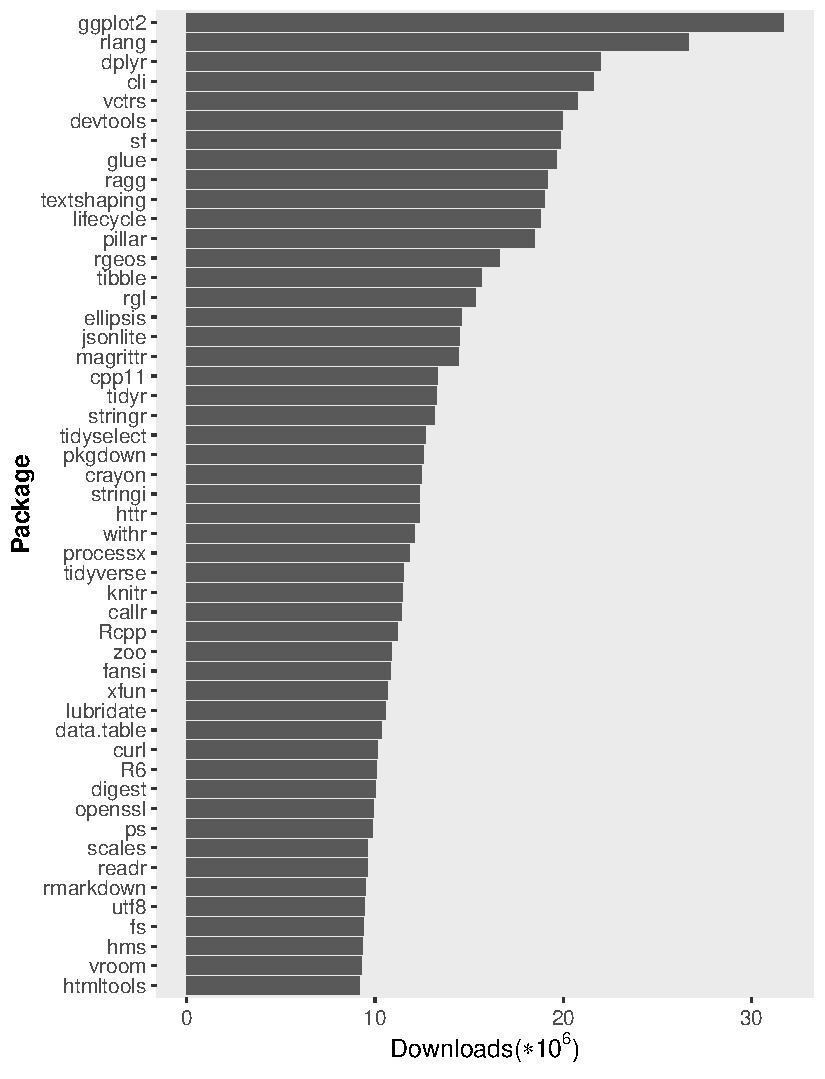
\includegraphics[width=9cm]{fig/downloads_50_plot.pdf}
    \caption{Top 50 packages downloaded on the RStudio mirror from 2021-11-01 to 2022-10-31.}

    \label{fig:download}
\end{figure}




\paragraph{Author Collaboration Network} Table~\ref{tab:rank_aut} lists the top 50 authors ranked by various indexes. RStudio is identified as the most influential author according to eigenvector and PageRank. Hadley Wickham and R Core demonstrated greatest influence based on degree and betweenness, respectively. Table~\ref{tab:rank2_aut} shows that 46 authors are ranked among the top 50 by at least two indexes, including organizations such as \href{https://www.r-project.org/contributors.html}{R Core}, RStudio, and Google Inc., as well as individual scientists affiliated with these organizations. Figure~\ref{fig:bipar} reveals that, unlike the base packages, most organizational authors of CRAN packages are not maintainers or creators. Instead, organizations such as RStudio acts as copyright holders and funders, and the R Core team often works as a contributor.

The results also suggest that different indexes prioritize different aspects of influence. Authors with limited but influential collaborators may not rank among the top 50 based on the degree centrality, but can be revealed using the eigenvector centrality and PageRank (Table~\ref{tab:rank_aut}). %This is because Eigenvector centrality and PageRank take the importance of neighbors into consideration when ranking nodes.


Table~\ref{tab:rank2_aut} presents the top downloaded packages of influential authors. Many packages have been identified as the influential packages listed in Table~\ref{tab:rank_pkg}. Figure~\ref{fig:cor_aut} shows the collaboration heatmap among these authors, revealing intensive collaboration among influential organizations and authors. The heatmap shows three main clusters of author collaboration. Most authors at the upper left corner of the heatmap (e.g., Dirk Eddelbuettel) have the same two packages \CRANpkg{DescTools} (an R package for descriptive statistics) and \CRANpkg{fortunes} (an R package of collected wisdom from the R community). Their co-authored packages are mainly about two main topics on {\it Data Import, Export, and Wrangling} (e.g., \CRANpkg{data.table}, \CRANpkg{MASS}) and {\it Data Visualization} (e.g., \CRANpkg{rgl}, \CRANpkg{plotrix}). Authors in the middle of the figure are clustered together because they co-authored the \CRANpkg{broom} package, a package for converting objects into tidy tibbles. Authors in the lower-right corner of the matrix co-authored many packages related to the {\it Data Visualization, Result Presentation, and Interactive Web Applications} topic (e.g., \CRANpkg{knitr}, \CRANpkg{bookdown}, \CRANpkg{shiny}), many of whom are from RStudio. These results align with to the finding in the package dependency network that many influential packages are related to the {\it Data Import, Export, and Wrangling} and {\it Data Visualization, Result Presentation, and Interactive Web Applications} topics.


\begin{figure}
\centering
    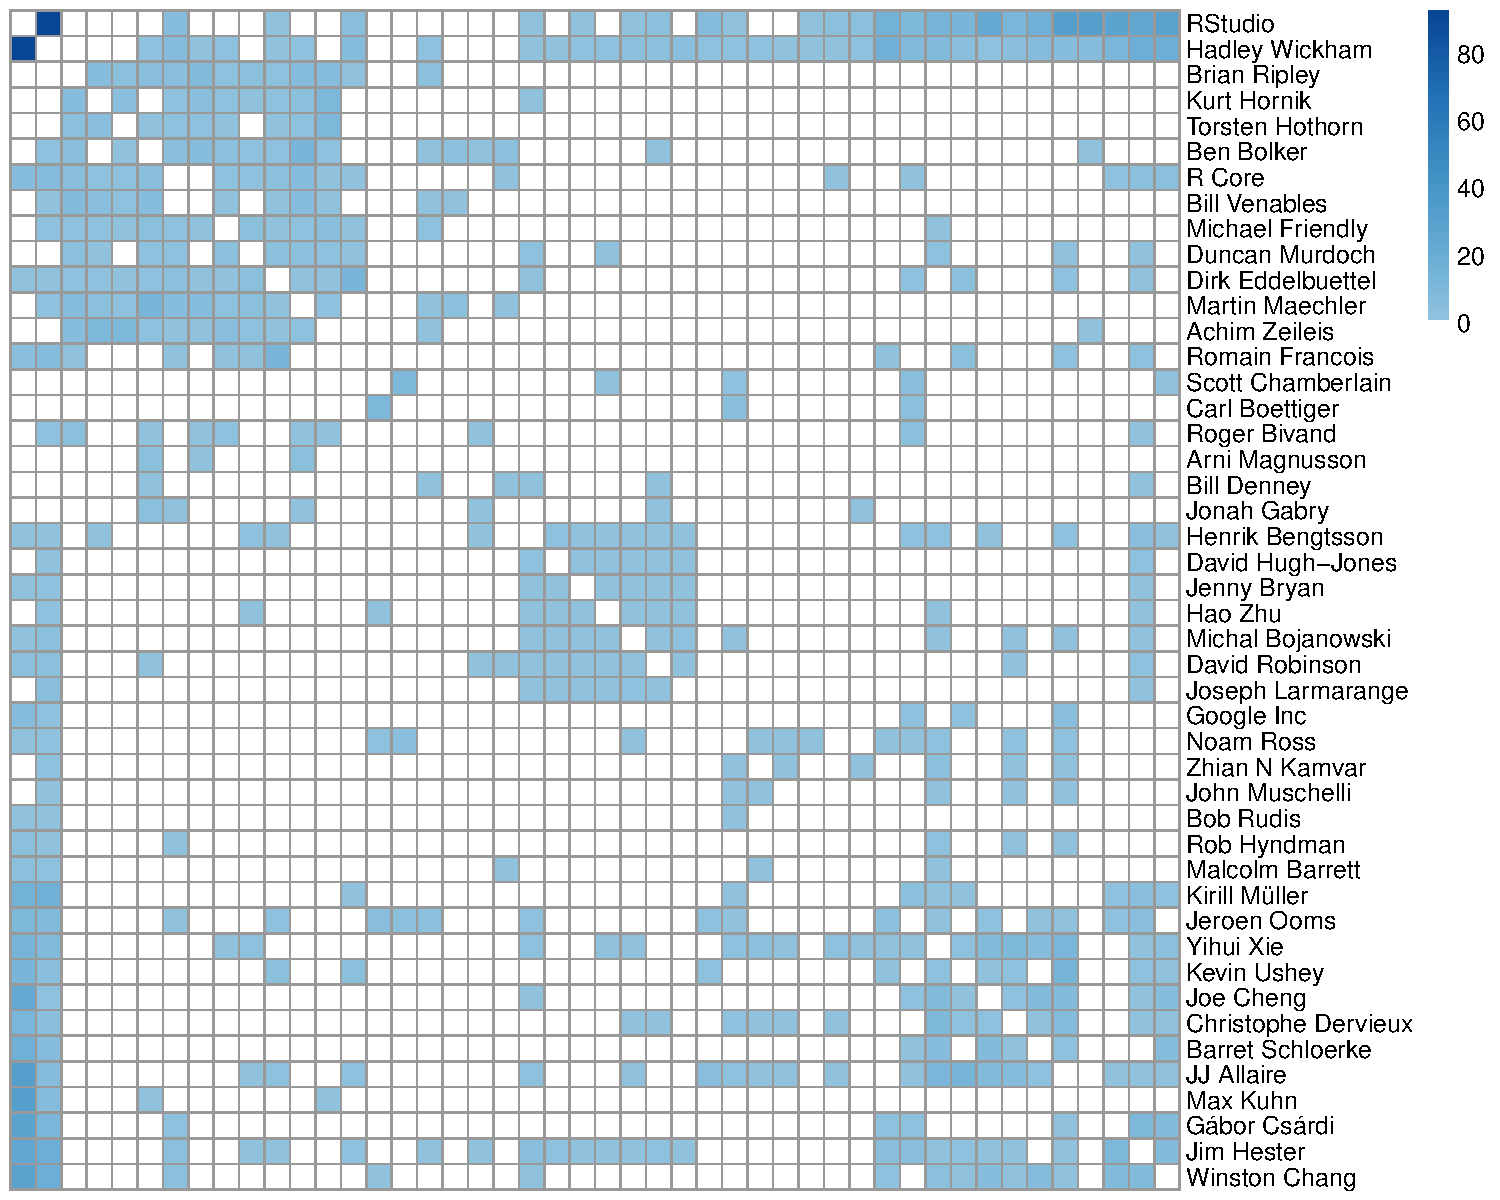
\includegraphics[width=15cm]{fig/cor_aut.pdf}
    \caption{Collaboration heatmap of the influential authors identified in the collaboration network.}

   {\small
\textit{Note.} Color denotes the number of co-authored packages between two authors.
}

    \label{fig:cor_aut}
\end{figure}



\paragraph{Bipartite Network} The BiRank values demonstrate small to medium correlations with the indexes used in the one-mode author collaboration network ($r=.179-.427$). The top 50 influential authors and their ranking are different from the results of the author collaboration network. Twenty-three of the top 50 authors are not ranked as top 50 by any index in the collaboration network (Table~\ref{tab:rank_bi_aut}). Compared to the influential authors in the collaboration network, these 23 authors' packages have relatively few number of authors. But the number of their packages is high. 

The most influential author identified by BiRank is Dirk Eddelbuettel, followed by Hadley Wickham, RStudio, Stéphane Laurent, and Scott Chamberlain. By contrast, in the one-mode network, Stéphane Laurent is not in the top 50 author lists based on degree, betweenness, and eigenvector. Scott Chamberlain is also not in the top 50 author lists based on degree and eigenvector. This is because many of their packages are solo-authored  (e.g., \CRANpkg{crul}). These results suggested that the bipartite network can identify productive and influential authors even without a high number of collaborators.



\section{Discussion}

The growing usage of R in data science is tightly associated with the increasing growth of the R ecosystem. With the rich amount of information on CRAN, this paper shows the main trends among the R developers and their packages.

Based on the package descriptions, we investigated the popular topics in the R ecosystem. Results identified a wide range of topics including various statistical methods (e.g., Cluster Analysis, Machine Learning, Bayesian Estimation, and Network Analysis) across different fields (e.g., Genetics, Environmetrics, Multivariate Analysis, and Psychometrics). Moreover, there were also packages for providing data sets, helping access to websites and online services, and improving computational efficiency. Some of these 19 topics are similar to the topics identified in the data science curricula \citep{zhang2021data} including {\it Machine Learning} and {\it Data Visualization, Result Presentation, and Interactive Web Applications}.

Using network analysis, we explored the influential packages and authors based on package dependencies and authorships. The results highlighted the crucial role of the base and recommended R packages in developing R packages, with 12 out of the 29 base and recommended packages ranked in the top 50 by at least two indexes. In addition to the packages shipped alongside base R, we also identified some important CRAN packages that support the development of R in various topics.  Many influential packages were related to {\it Data Visualization, Result Presentation, and Interactive Web Applications} and {\it Data Import, Export, and Wrangling} topics. These results were similar to the finding that influential authors co-developed many important packages of these two topics. 

Our findings also indicated that the contributors of R, developing from the R Core team, now have become a worldwide community, and some of them are organizations. Many of these influential authors are from RStudio or the R Core team and lead the development across many topics. For example, Yihui Xie, the creator of \CRANpkg{knitr} and many R markdown-related packages, facilitates the development of reproducible research. While some of these influential contributors are from central positions in the author collaboration network, we also identified many productive authors with relatively few collaborators through the bipartite network of packages and authors.

\subsection{Limitations and Future Directions}

There are a few of limitations in the current work. First, we investigated the influential packages from the perspective of the developer community rather than the user community. To illustrate, we focused on identifying which packages are used by other packages (i.e., in the package dependency network). However, packages with high influence for developers may differ from those for the user community. Future studies are needed to explore important packages based on the usage data (e.g., citations, number of times mentioned on Twitter). Second, package dependency relationships cannot distinguish between dependencies required for publishing the package, such as vignette generation, and those needed for developing utilities. To better understand the relationships of packages based on their functionality, future study can explore the similarity between packages based on text analysis of reference manuals or vignettes. Third, we only included the R packages on CRAN or embedded in the R source code. There has already been a trend of releasing packages on GitHub and R-universe (a personal R package repository). Numerous GitHub packages and their information (e.g., contributors, commits, stars, forks) could be a rich resource for future research to understand the development and importance of R packages. Forth, as suggested by a referee, future studies can compare R and other software communites (e.g., Python). Fifth, this paper was limited by the timing of data extraction and did not include the state of the R community in the past. Future research are suggested to conduct longitudinal analysis of the R community to understand how it developed over time.

This paper also provides directions for the development of an R package recommendation system.   As \citet{RJ-2018-058} suggested, with the growth of the R ecosystems, it becomes difficult for the users to search for specific packages on CRAN. The flat organization of R packages, as well as the sorting system based on name or the date of publication, pose a big challenge for searching. It has been proposed to add keywords or tags for packages to help organize and search packages \citep{RJ-2018-058}.  Based on the results of the current paper, future research is suggested to develop a package recommendation system using the information on CRAN. Specifically, the topic modeling can help identify packages related to different topics and could also be an effective way for automatically tagging. Network analysis can also help understand the relationships among packages. Methods based on network analysis such as latent space modeling may help quantify the closeness of two packages and provide recommendations.


\subsection{Concluding Remarks}

This paper depicts a general picture of the R developer community based on information on CRAN. Results identified the popular topics of the R ecosystem. Investigation of influential packages and authors also contributes to the understanding of the development of the R community. It is the efforts from these experts with various backgrounds that lead to the prosperity of the R ecosystem. Moreover, results of the current study highlight the direction for developing a package recommendation system.


\subsection{Acknowledgment}

This work is supported by a grant from the Department of Education (R305D210023) and the Notre Dame International at the University of Notre Dame. However, the contents of the study do not necessarily represent the policy of the Department of Education, and you should not assume endorsement by the Federal Government.

\appendix

\section{Appendix}
\setcounter{table}{0}
\renewcommand{\thetable}{A\arabic{table}}
\begin{table}[h]
\tabcolsep 2pt \caption{Top 50 packages identified based on different network statistics of the package dependency network.} \vspace{0.0in}
\begin{center} \label{tab:rank_pkg}
\resizebox{0.6\textwidth}{!}{
\begin{tabular}{llllllllll}
\toprule
Rank  & In-degree & Betweenness & Eigenvector  & PageRank \\
 \midrule
 1 & knitr & ggplot2 & knitr & testthat \\
 2 & testthat & knitr & rmarkdown & utils \\
 3 & rmarkdown & broom & testthat & methods \\
 4 & stats & dplyr & stats & stats \\
 5 & Rcpp & emmeans & ggplot2 & knitr \\
 6 & ggplot2 & testthat & dplyr & patchSynctex \\
 7 & methods & shiny & methods & rmarkdown \\
 8 & dplyr & stats & utils & tools \\
 9 & utils & rmarkdown & Rcpp & covr \\
 10 & graphics & survival & rlang & stringr \\
 11 & MASS & bayestestR & magrittr & graphics \\
 12 & magrittr & sf & tibble & mapmisc \\
 13 & covr & gap & tidyr & Rcpp \\
 14 & rlang & MASS & graphics & tis \\
 15 & tibble & targets & covr & grDevices \\
 16 & tidyr & caret & stringr & rlang \\
 17 & stringr & multcomp & purrr & MASS \\
 18 & grDevices & Hmisc & MASS & ggplot2 \\
 19 & purrr & texreg & grDevices & magrittr \\
 20 & parallel & insight & data.table & withr \\
 21 & Matrix & parameters & jsonlite & jsonlite \\
 22 & data.table & enrichwith & Matrix & parallel \\
 23 & jsonlite & cops & shiny & htmltools \\
 24 & RcppArmadillo & mlr & parallel & scales \\
 25 & shiny & zoo & httr & fastcluster \\
 26 & httr & earth & glue & enrichwith \\
 27 & mvtnorm & tibble & scales & cops \\
 28 & survival & AER & sf & QuasiSeq \\
 29 & foreach & lme4 & readr & tibble \\
 30 & scales & jsonlite & lubridate & dplyr \\
 31 & plyr & robustbase & igraph & lattice \\
 32 & igraph & plotmo & reshape2 & plyr \\
 33 & reshape2 & quantreg & withr & R6 \\
 34 & lubridate & effects & gridExtra & vctrs \\
 35 & doParallel & rgl & foreach & reshape \\
 36 & grid & nnet & cli & glue \\
 37 & sp & nlme & tidyselect & digest \\
 38 & gridExtra & sp & plyr & tinytest \\
 39 & readr & doParallel & xml2 & RUnit \\
 40 & spelling & surveillance & sp & httr \\
 41 & lattice & mice & plotly & Matrix \\
 42 & glue & Matrix & grid & xml2 \\
 43 & RColorBrewer & data.tree & survival & shiny \\
 44 & sf & car & lme4 & curl \\
 45 & xml2 & spelling & vctrs & rstudioapi \\
 46 & raster & metafor & lifecycle & cli \\
 47 & zoo & marginaleffects & broom & yaml \\
 48 & markdown & gtools & mvtnorm & survival \\
 49 & R6 & partykit & RcppArmadillo & markdown \\
 50 & glmnet & hunspell & doParallel & htmlwidgets \\
\bottomrule
\end{tabular}
}
\end{center}
\end{table}


	
\clearpage	
\newpage
\begin{table}[h]
\tabcolsep 2pt \caption{Packages identified by at least two indexes.} \vspace{0.0in}
\begin{center} \label{tab:rank2_pkg}
\resizebox{\textwidth}{!}{
\begin{tabular}{llllll}
\toprule
Package  & Title & Maintainer\\
 \midrule
 knitr & A General-Purpose Package for Dynamic Report Generation in R & Yihui Xie \\
 ggplot2 & Create Elegant Data Visualisations Using the Grammar of Graphics & Thomas Lin Pedersen \\
 testthat & Unit Testing for R & Hadley Wickham \\
 rmarkdown & Dynamic Documents for R & Yihui Xie \\
 utils* & 	The R Utils Package & R Core  \\
 broom & Convert Statistical Objects into Tidy Tibbles & Simon Couch \\
 methods* & Formal Methods and Classes &  R Core  \\
 stats* & The R Stats Package & R Core  \\
 dplyr & A Grammar of Data Manipulation & Hadley Wickham \\
 Rcpp & Seamless R and C++ Integration & Dirk Eddelbuettel \\
 shiny & Web Application Framework for R & Winston Chang \\
 covr & Test Coverage for Packages & Jim Hester \\
 grDevices* & The R Graphics Devices and Support for Colours and Fonts &  R Core \\
 survival & Survival Analysis & Terry M Therneau \\
 rlang & Functions for Base Types and Core R and 'Tidyverse' Features & Lionel Henry \\
 stringr & Simple, Consistent Wrappers for Common String Operations & Hadley Wickham \\
 MASS* & Support Functions and Datasets for Venables and Ripley's MASS & Brian Ripley \\
 magrittr & A Forward-Pipe Operator for R & Lionel Henry \\
 sf & Simple Features for R & Edzer Pebesma \\
 tibble & Simple Data Frames & Kirill Müller \\
 tidyr & Tidy Messy Data & Hadley Wickham \\
 graphics* & The R Graphics Package &  R Core \\
 purrr & Functional Programming Tools & Lionel Henry \\
 parallel* & Support for Parallel Computation & R Core \\
 data.table & Extension of `data.frame` & Matt Dowle \\
 withr & Run Code 'With' Temporarily Modified Global State & Lionel Henry \\
 Matrix* & Sparse and Dense Matrix Classes and Methods & Martin Maechler \\
 jsonlite & A Simple and Robust JSON Parser and Generator for R & Jeroen Ooms \\
 enrichwith & Methods to Enrich R Objects with Extra Components & Ioannis Kosmidis \\
 cops & Cluster Optimized Proximity Scaling & Thomas Rusch \\
 RcppArmadillo & Rcpp' Integration for the 'Armadillo' Templated Linear Algebra Library & Dirk Eddelbuettel \\
 scales & Scale Functions for Visualization & Hadley Wickham \\
 zoo & S3 Infrastructure for Regular and Irregular Time Series (Z's Ordered Observations) & Achim Zeileis \\
 httr & Tools for Working with URLs and HTTP & Hadley Wickham \\
 glue & Interpreted String Literals & Jennifer Bryan \\
 mvtnorm & Multivariate Normal and t Distributions & Torsten Hothorn \\
 foreach & Provides Foreach Looping Construct & Folashade Daniel \\
 lme4 & Linear Mixed-Effects Models using 'Eigen' and S4 & Ben Bolker \\
 readr & Read Rectangular Text Data & Jennifer Bryan \\
 lubridate & Make Dealing with Dates a Little Easier & Vitalie Spinu \\
 plyr & Tools for Splitting, Applying and Combining Data & Hadley Wickham \\
 igraph & Network Analysis and Visualization & Tamás Nepusz \\
 lattice* & Trellis Graphics for R & Deepayan Sarkar \\
 reshape2 & Flexibly Reshape Data: A Reboot of the Reshape Package & Hadley Wickham \\
 R6 & Encapsulated Classes with Reference Semantics & Winston Chang \\
 gridExtra & Miscellaneous Functions for "Grid" Graphics & Baptiste Auguie \\
 vctrs & Vector Helpers & Lionel Henry \\
 doParallel & Foreach Parallel Adaptor for the 'parallel' Package & Folashade Daniel \\
 grid* & The Grid Graphics Package &  R Core \\
 cli & Helpers for Developing Command Line Interfaces & Gábor Csárdi \\
 sp & Classes and Methods for Spatial Data & Edzer Pebesma \\
 xml2 & Parse XML & Hadley Wickham \\
 spelling & Tools for Spell Checking in R & Jeroen Ooms \\
 markdown & Render Markdown with 'commonmark' & Yihui Xie \\
\bottomrule
\end{tabular}
}

{\small
\textit{Note.} *\href{https://stat.ethz.ch/R-manual/R-devel/doc/html/packages.html}{Base and recommended R packages} are part of R source code.
}
\end{center}
\end{table}


\clearpage
\newpage
\begin{table}[h]
\tabcolsep 2pt  \caption{Top 50 authors identified based on different network statistics of the author collaboration network.} \vspace{0.0in}
\begin{center} \label{tab:rank_aut}
\resizebox{1\columnwidth}{!}{
\begin{tabular}{llllllllll}
\toprule
Rank & Degree & Betweenness & Eigenvector & PageRank  \\
 \midrule
 1 & Hadley Wickham & R Core & RStudio & RStudio \\
 2 & RStudio & Hadley Wickham & Hadley Wickham & Hadley Wickham \\
 3 & Dirk Eddelbuettel & Dirk Eddelbuettel & Jim Hester & R Core \\
 4 & Ben Bolker & Martin Maechler & JJ Allaire & Martin Maechler \\
 5 & R Core & RStudio & Winston Chang & Ben Bolker \\
 6 & Martin Maechler & Ben Bolker & Yihui Xie & Dirk Eddelbuettel \\
 7 & Yihui Xie & Kurt Hornik & Joe Cheng & Yihui Xie \\
 8 & Brian Ripley & Brian Ripley & Max Kuhn & Achim Zeileis \\
 9 & Michael Friendly & Roger Bivand & Gábor Csárdi & JJ Allaire \\
 10 & Jim Hester & Achim Zeileis & Lionel Henry & Kurt Hornik \\
 11 & Roger Bivand & Scott Chamberlain & Kirill Müller & Brian Ripley \\
 12 & JJ Allaire & Jeroen Ooms & Kevin Ushey & Roger Bivand \\
 13 & Henrik Bengtsson & Yihui Xie & Christophe Dervieux & Jim Hester \\
 14 & Bill Venables & Zhian N Kamvar & Barret Schloerke & Jeroen Ooms \\
 15 & Kevin Ushey & Michael Friendly & Jennifer Bryan & Scott Chamberlain \\
 16 & Achim Zeileis & John Muschelli & Jeroen Ooms & Michael Friendly \\
 17 & Kurt Hornik & Rob Hyndman & Carson Sievert & Zhian N Kamvar \\
 18 & Max Kuhn & Tyler Rinker & Javier Luraschi & Winston Chang \\
 19 & Romain Francois & Bill Denney & Romain Francois & Joe Cheng \\
 20 & Duncan Murdoch & John Wiseman & Daniel Falbel & Henrik Bengtsson \\
 21 & Zhian N Kamvar & Thomas Lumley & PBC & Bob Rudis \\
 22 & David Robinson & Jim Hester & R Core & Kevin Ushey \\
 23 & Hao Zhu & Sahir Bhatnagar & Henrik Bengtsson & Duncan Murdoch \\
 24 & Michal Bojanowski & Henrik Bengtsson & Ben Bolker & Max Kuhn \\
 25 & Joe Cheng & Toby Hocking & David Robinson & Bill Venables \\
 26 & Vilmantas Gegzna & Carl Boettiger & Michal Bojanowski & John Muschelli \\
 27 & Christophe Dervieux & Kevin Ushey & Thomas Lin Pedersen & Gábor Csárdi \\
 28 & Bill Denney & Kirill Müller & Davis Vaughan & Rob Hyndman \\
 29 & Adrian Baddeley & Bob Rudis & JooYoung Seo & Torsten Hothorn \\
 30 & Jeroen Ooms & Cleve Moler & Atsushi Yasumoto & Kirill Müller \\
 31 & Hong Ooi & JJ Allaire & Yixuan Qiu & Noam Ross \\
 32 & Noam Ross & Noam Ross & Joseph Larmarange & Romain Francois \\
 33 & David Hugh-Jones & Bill Venables & Dirk Eddelbuettel & Christophe Dervieux \\
 34 & Joseph Larmarange & Max Kuhn & Malcolm Barrett & Carl Boettiger \\
 35 & John Muschelli & Ben Goodrich & Noam Ross & David Robinson \\
 36 & Jonah Gabry & Jonah Gabry & Jeff Allen & Jonah Gabry \\
 37 & Malcolm Barrett & Christophe Dutang & Hao Zhu & Maëlle Salmon \\
 38 & Greg Snow & Torsten Hothorn & Michael Friendly & Michael Sumner \\
 39 & Jim Lemon & Winston Chang & Jenny Bryan & Barret Schloerke \\
 40 & Alessandro Gasparini & Kosuke Imai & Google Inc & Stéphane Laurent \\
 41 & Eduard Szoecs & Apache Foundation & David Hugh-Jones & Bill Denney \\
 42 & Tal Galili & Arni Magnusson & jQuery Foundation & Edzer Pebesma \\
 43 & Jenny Bryan & Romain Francois & Roger Bivand & Hao Zhu \\
 44 & Torsten Hothorn & Joe Cheng & Hiroaki Yutani & Indrajeet Patil \\
 45 & Matthieu Stigler & Duncan Murdoch & Martin Maechler & Michel Lang \\
 46 & Garrick Aden-Buie & Steven G Johnson & Alex Hayes & Michal Bojanowski \\
 47 & Dieter Menne & Yuan Tang & Mango Solutions & John Fox \\
 48 & Frank E Harrell Jr & Jacob Bien & Richard Iannone & Google Inc \\
 49 & Rolf Turner & Lampros Mouselimis & Simon Couch & Arni Magnusson \\
 50 & Michael Chirico & Yi Yang & Frederik Aust & Uwe Ligges \\
\bottomrule
\end{tabular}
}
\end{center}
\end{table}

	

\clearpage	
\newpage
\fancyheadoffset{2cm}
\begin{table}[h]
\tabcolsep 2pt \caption{Authors identified by at least two indexes.} \vspace{0.0in}
\begin{center} \label{tab:rank2_aut}
\resizebox{.75\columnwidth}{!}{
\begin{tabular}{llll}
\toprule
Author  & His or Her top downloaded packages \\
 \midrule
 Hadley Wickham & ggplot2, rlang, dplyr, cli, vctrs \\
 R Core & rgl, fansi, testthat, pkgload, car \\
 RStudio & ggplot2, rlang, dplyr, cli, vctrs \\
 Dirk Eddelbuettel & rgl, Rcpp, data.table, digest, nloptr \\
 Jim Hester & devtools, glue, cpp11, withr, knitr \\
 Ben Bolker & rgl, broom, lme4, car, gtools \\
 Martin Maechler & lme4, car, bitops, MatrixModels, mvtnorm \\
 JJ Allaire & knitr, Rcpp, rmarkdown, rstudioapi, shiny \\
 Winston Chang & ggplot2, devtools, withr, processx, callr \\
 Yihui Xie & knitr, xfun, rmarkdown, htmltools, yaml \\
 Kurt Hornik & digest, colorspace, nloptr, e1071, tseries \\
 Joe Cheng & knitr, rmarkdown, htmltools, bslib, sass \\
 Brian Ripley & nloptr, car, bit, quantreg, MASS \\
 Max Kuhn & broom, generics, caret, recipes, hardhat \\
 Achim Zeileis & zoo, colorspace, car, lmtest, quantreg \\
 Michael Friendly & knitr, car, maptools, DescTools, vcd \\
 Roger Bivand & sf, rgeos, broom, sp, maptools \\
 Gábor Csárdi & cli, rgl, crayon, processx, callr \\
 Scott Chamberlain & plotly, crul, httpcode, jqr, bibtex \\
 Kirill Müller & dplyr, cli, sf, pillar, tibble \\
 Jeroen Ooms & sf, rgl, jsonlite, curl, openssl \\
 Kevin Ushey & withr, Rcpp, data.table, rmarkdown, rstudioapi \\
 Henrik Bengtsson & knitr, digest, broom, globals, matrixStats \\
 Christophe Dervieux & knitr, xfun, rmarkdown, sass, tinytex \\
 Bill Venables & MASS, raster, polynom, gplots, plotrix \\
 Zhian N Kamvar & knitr, yaml, ggrepel, adegenet, rticles \\
 Barret Schloerke & rmarkdown, htmltools, evaluate, sass, shiny \\
 John Muschelli & knitr, officer, rticles, riskRegression, rscopus \\
 Rob Hyndman & rmarkdown, forecast, fracdiff, tsfeatures, tsibble \\
 Romain Francois & tibble, knitr, Rcpp, readr, RcppEigen \\
 Bill Denney & digest, broom, classInt, janitor, rio \\
 Duncan Murdoch & rgl, knitr, digest, car, kableExtra \\
 Bob Rudis & viridisLite, viridis, ggthemes, hrbrthemes, flexdashboard \\
 David Robinson & knitr, broom, reprex, tidytext, broom.mixed \\
 Hao Zhu & knitr, broom, kableExtra, skimr, REDCapR \\
 Michal Bojanowski & knitr, broom, labelled, bookdown, alluvial \\
 Carl Boettiger & rticles, EML, taxize, drat, RNeXML \\
 Torsten Hothorn & lmtest, mvtnorm, ipred, multcomp, TH.data \\
 Noam Ross & knitr, viridisLite, viridis, bookdown, data.tree \\
 Joseph Larmarange & knitr, lubridate, broom, GGally, labelled \\
 David Hugh-Jones & knitr, broom, covr, maxLik, huxtable \\
 Malcolm Barrett & rmarkdown, broom, ggrepel, usethis, bayesplot \\
 Jonah Gabry & broom, rstan, StanHeaders, loo, rstantools \\
 Jenny Bryan & knitr, broom, tidyxl \\
 Google Inc & rmarkdown, gargle, s2, odbc, tensorflow \\
 Arni Magnusson & xtable, gplots, coda, gdata, DescTools \\
\bottomrule
\end{tabular}}
\end{center}
\end{table}



\clearpage	
\newpage
\fancyheadoffset{2cm}
\begin{table}[h]
\tabcolsep 2pt \caption{Authors identified in the bipartite network and not in the author collaboration network.} \vspace{0.0in}
\begin{center} \label{tab:rank_bi_aut}
\resizebox{1.05\columnwidth}{!}{
\begin{tabular}{llll}
\toprule
Author  & His or Her top downloaded packages \\
\midrule
Jan Wijffels & imager, udpipe, cronR, taskscheduleR, opencv\\
Robin K S Hankin & gsl, hypergeo, elliptic, contfrac, magic\\
Simon Urbanek & rgl, digest, base64enc, uuid, rJava\\
Kartikeya Bolar & STAT, ANOVAIREVA, ANOVAShiny, ANOVAShiny2, BLRShiny\\
Richard Cotton & withr, knitr, assertive.properties, assertive.base, assertive\\
Muhammad Yaseen & PakPMICS2014HL, PakPMICS2014Wm, DiallelAnalysisR, bayesammi, baystability\\
Guangchuang Yu & yulab.utils, ggfun, aplot, ggplotify, tidytree\\
Florian Schwendinger & Rglpk, lpSolveAPI, ROI, scs, Rsymphony\\
Paul Murrell & colorspace, lattice, polyclip, gridGraphics, gridBase\\
Kisung You & Rdimtools, maotai, mclustcomp, ADMM, ROptSpace\\
Przemyslaw Biecek & survminer, DALEX, iBreakDown, ingredients, eurostat\\
Joe Thorley & chk, yesno, nlist, term, universals\\
Philippe Grosjean & Rcmdr, sfsmisc, pastecs, tcltk2, svDialogs\\
Mohamed El Fodil Ihaddaden & ggeasy, ralger, BARIS, batata, bubblyr\\
Karline Soetaert & shape, inline, DescTools, deSolve, rootSolve\\
Emil Hvitfeldt & tidytext, yardstick, parsnip, prismatic, themis\\
Kevin R Coombes & ClassDiscovery, oompaBase, PCDimension, oompaData, Polychrome\\
Matthias Kohl & DescTools, distr, distrEx, MKmisc, MKinfer\\
Michael Hahsler & dbscan, arules, arulesSequences, seriation, TSP\\
Michael Kleinsasser & AEenrich, covid19india, SEIRfansy, eSIR, FEprovideR\\
Robrecht Cannoodt & ggrepel, rticles, proxyC, princurve, diffusionMap\\
Pablo Sanchez & facebookadsR, googleadsR, pinterestadsR, linkedInadsR, campaignmanageR\\
Paul R Rosenbaum & sensitivityfull, sensitivitymw, sensitivitymv, sensitivitymult, exteriorMatch\\
\bottomrule
\end{tabular}}
\end{center}
\end{table}





\hypertarget{refs}{}

\bibliography{pkg.bib}

\address{%
Lijin Zhang\\
Graduate School of Education, Stanford University\\%
United States\\
%
%
\textit{ORCiD: \href{https://orcid.org/0000-0002-4222-8850}{0000-0002-4222-8850}}\\%
\href{mailto:lijinzhang@stanford.edu}{\nolinkurl{lijinzhang@stanford.edu}}%
}

\address{%
Xueyang Li\\
Department of Computer Science and Engineering, University of Notre
Dame\\%
United States\\
%
%
%
\href{mailto:xli34@nd.edu}{\nolinkurl{xli34@nd.edu}}%
}

\address{%
Zhiyong Zhang\\
Department of Psychology, University of Notre Dame\\%
United States\\
%
%
\textit{ORCiD: \href{https://orcid.org/0000-0003-0590-2196}{0000-0003-0590-2196}}\\%
\href{mailto:zzhang4@nd.edu}{\nolinkurl{zzhang4@nd.edu}}%
}
